\chapter{Case study}
\section{Glyph tracking}
\subsection{Background}

The norm in the industry is that CCTV cameras are manually selected depending on needs, usually through using touch screens that display a set of four pictures at once. They are controllable through PTZ, but they are usually only moved to preset locations, by navigating the user interface.

\begin{figure}[ht]
    \centering
    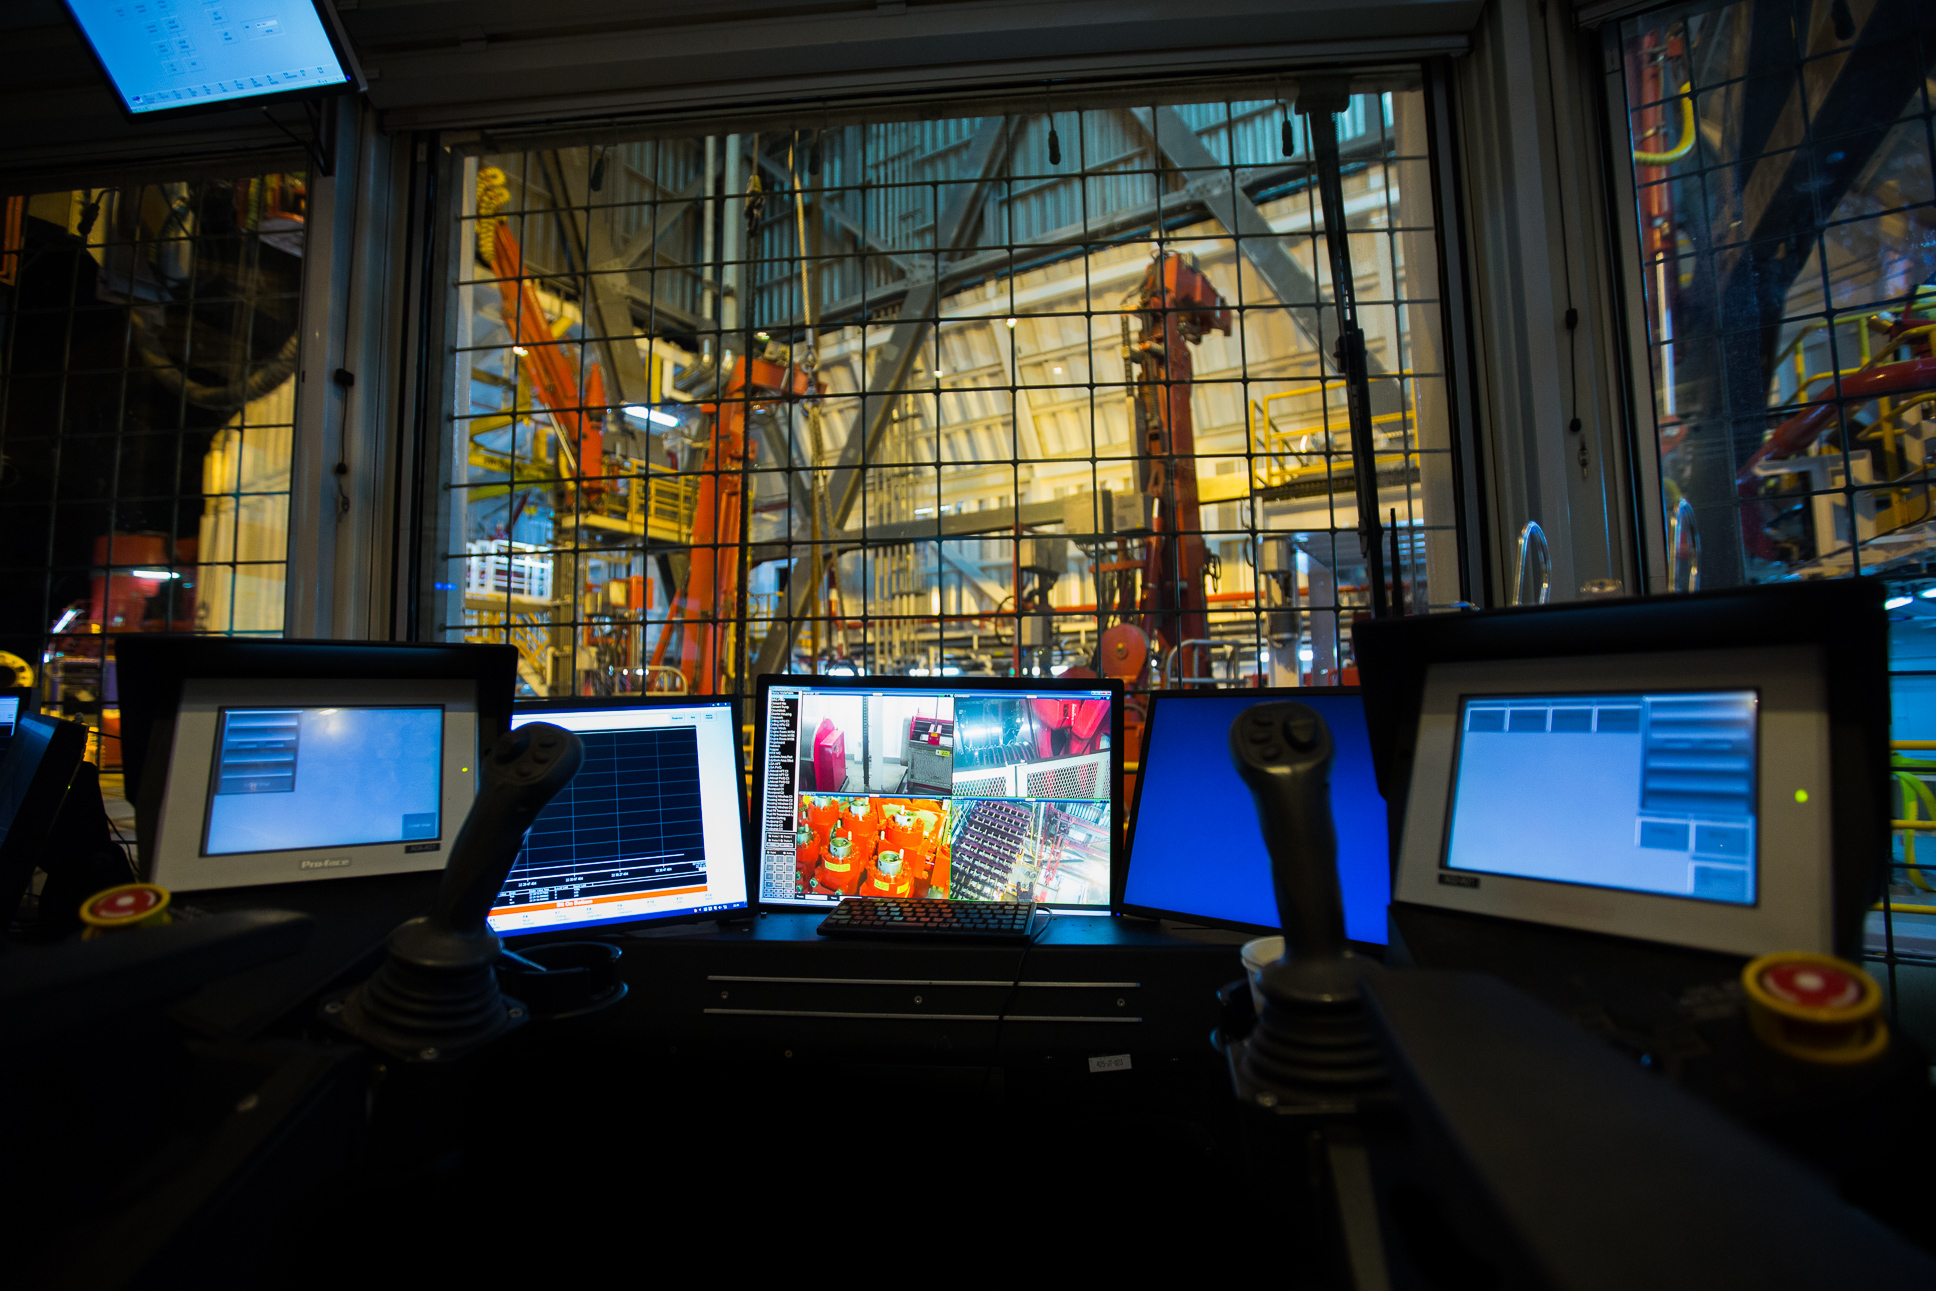
\includegraphics[width=1.0\textwidth]{VHA_4389_retouched.jpg}
    \caption{Modern driller cabin. Credit: Vegard Haugland, MHWirth AS, \citet{hauglandfoto15}}
    \label{fig:driller_cabin}
\end{figure}
\FloatBarrier

\subsection{Goal of case study}
This case study is intended to further improve upon the work done in the unpublished project thesis covering work done by the author in the year 2014. \citet{joakimsk14} describes the original idea, but it is briefly repeated here for brevity.

Through the detection and tracking of simple symbols attached to heavy machinery on an oil rig, it is possible to allow CCTV cameras to follow machines without any extra user input. These simple symbols are called "glyphs", and their design is chosen so to reduce processing requirements and increasing possibility of detection by the algorithm.

The case study described in \citet{joakimsk14} was implemented in an interpreted programming language Python 2.7 using OpenCV 2.4, while this new implementation is being written in a compiled programming language C++11 using OpenCV 3.0, which was recently released.

\begin{figure}[ht]
    \centering
    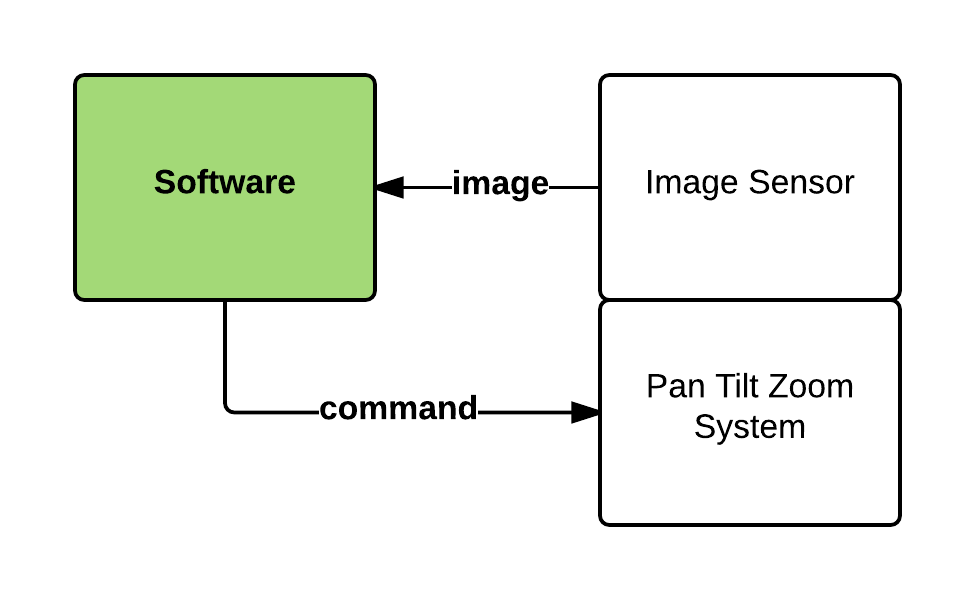
\includegraphics[width=0.8\textwidth]{cfs_simple_new.png}
    \caption{System overview using a single camera. Source:Own work, based on \citet{joakimsk14}}
    \label{fig:cfs_simple_new}
\end{figure}
\FloatBarrier

The simple system as shown in figure \ref{fig:cfs_simple_new} can be extended to use multiple sources. We extend the system to fulfill its role on an imaginary oil rig, where it allows the drillers to easily follow a moving top drive.

\begin{figure}[ht]
    \centering
    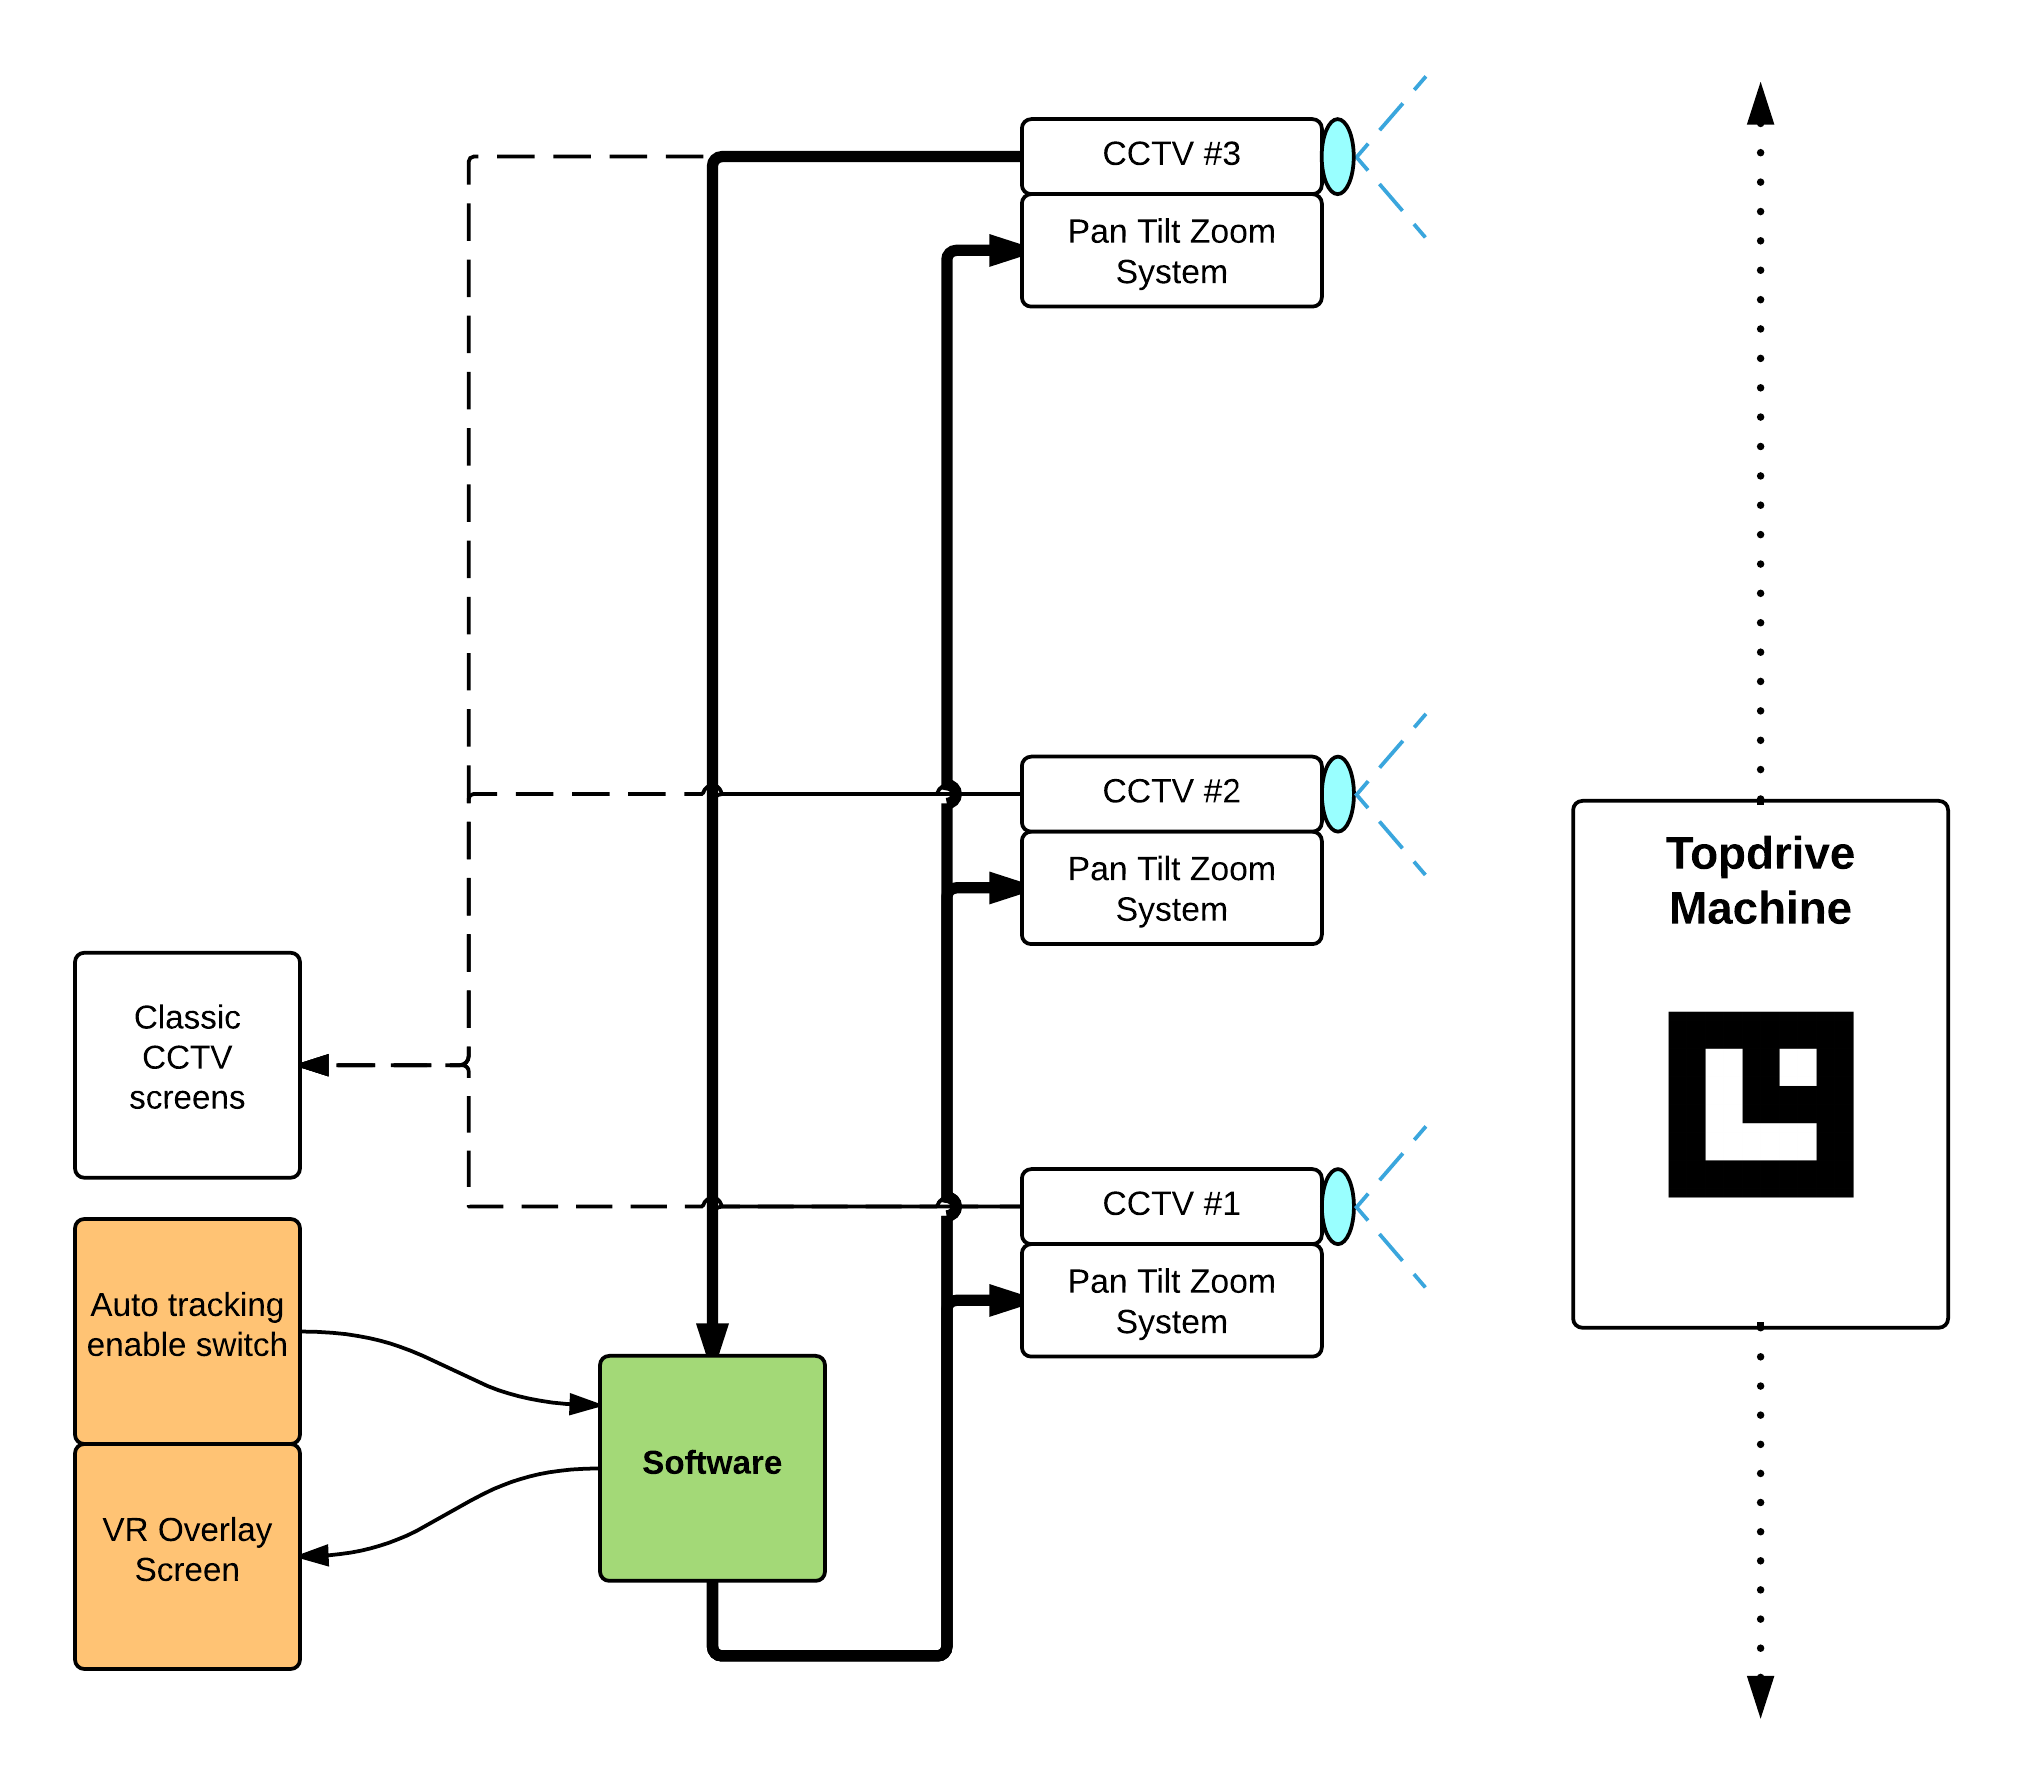
\includegraphics[width=0.8\textwidth]{cfs_system_rig.png}
    \caption{System overview when used on an oil rig. Source: Own work}
    \label{fig:cfs_system_rig}
\end{figure}
\FloatBarrier

With the software in place, controlling several CCTV cameras as shown in figure \ref{fig:cfs_system_rig}, we hope to allow the control loop to quickly and efficiently follow the machine as it moves about. 

At the end of this case study, we will see a side-by-side comparison of the old and new implementation, and consider differences in performance.

\subsection{Design of the machine vision algorithm}
The machine vision algorithm remains the same as earlier developed, as to give us equal grounds for comparison. There are steps that can improve detection rate and reduce processing requirements which will be mentioned, but not necessarily implemented. For details about the algorithm described in figure \ref{fig:cva_detail}, please refer to the unpublished project thesis by the author \citep{joakimsk14}.

\begin{figure}[ht]
    \centering
    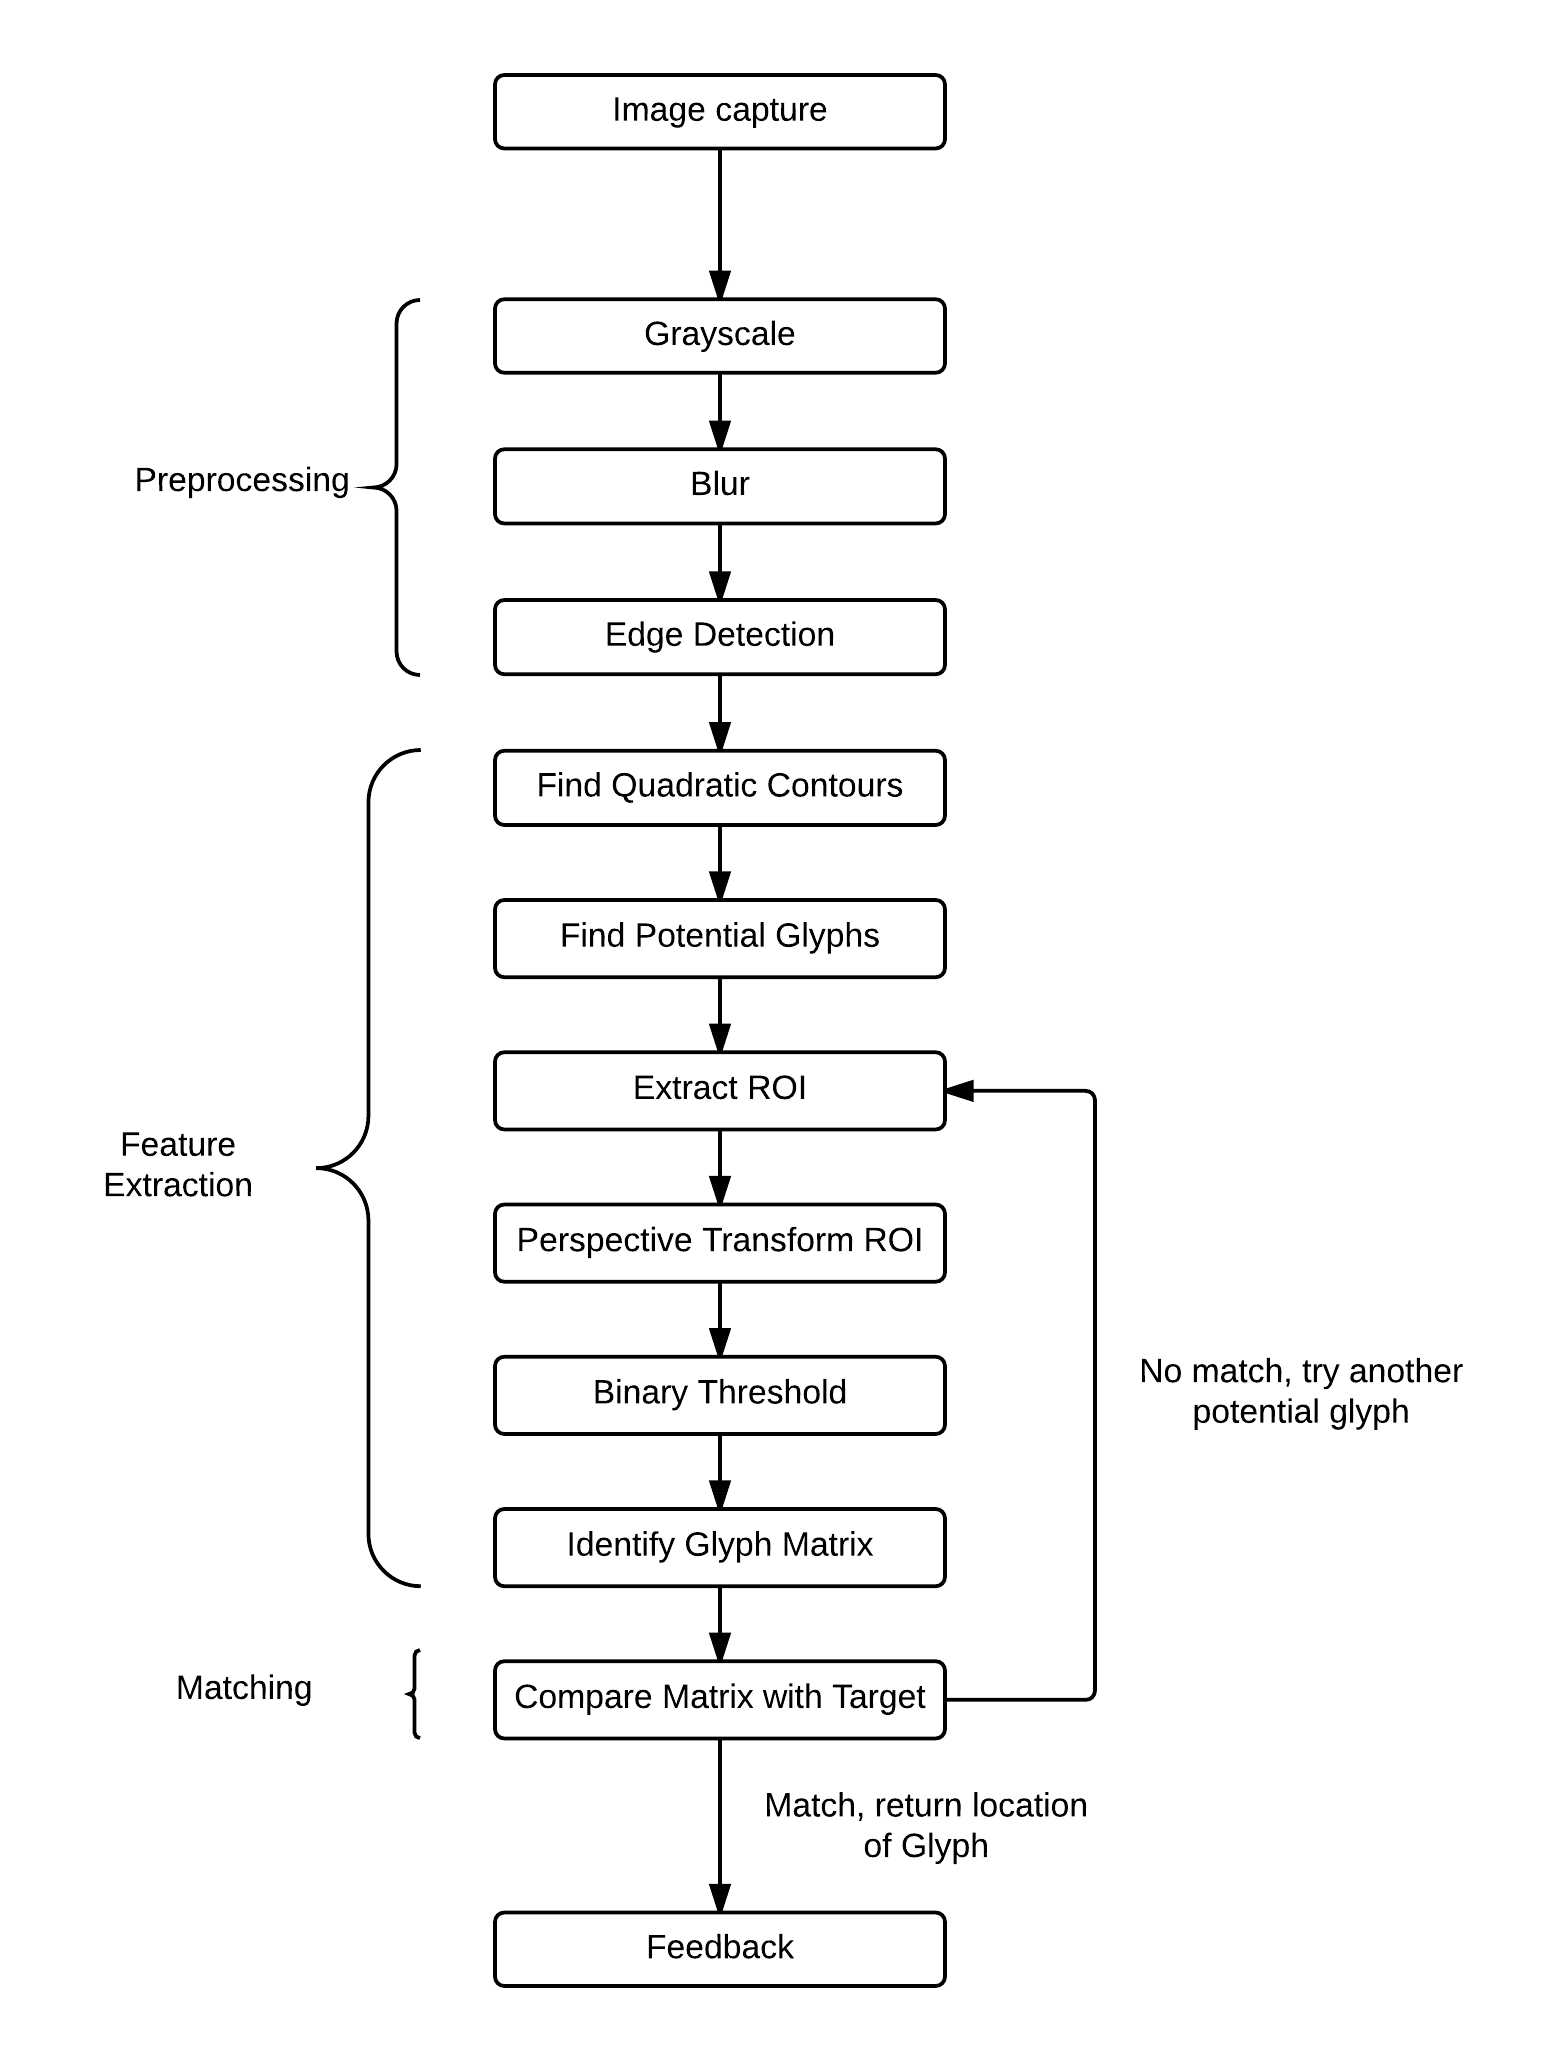
\includegraphics[width=0.8\textwidth]{cva_detail.png}
    \caption{The vision algorithm as implemented. Source:\citet{joakimsk14}}
    \label{fig:cva_detail}
\end{figure}
\FloatBarrier

\subsection{Design of the software}
Using C++11, the software is expected to run faster than the similar Python 2.7-version implemented in \citet{joakimsk14}. When we have OpenCL-support in hardware, a greater speedup is expected to be seen for parts of the machine vision algorithm.

The software is designed to run in a single thread, despite of potential benefits from using multiple threads as described in Chapter \ref{ch:chapter2}, because of difficulties with making a multithreaded application behave as expected. This also means that the comparison between the Python 2.7-version and the C++11-version stands on equal ground. A flowchart of the software as a single thread can be seen in figure \ref{fig:software_design}, where the machine vision algorithm is implemented inside Camera.FindGlyph().

\begin{figure}[ht]
    \centering
    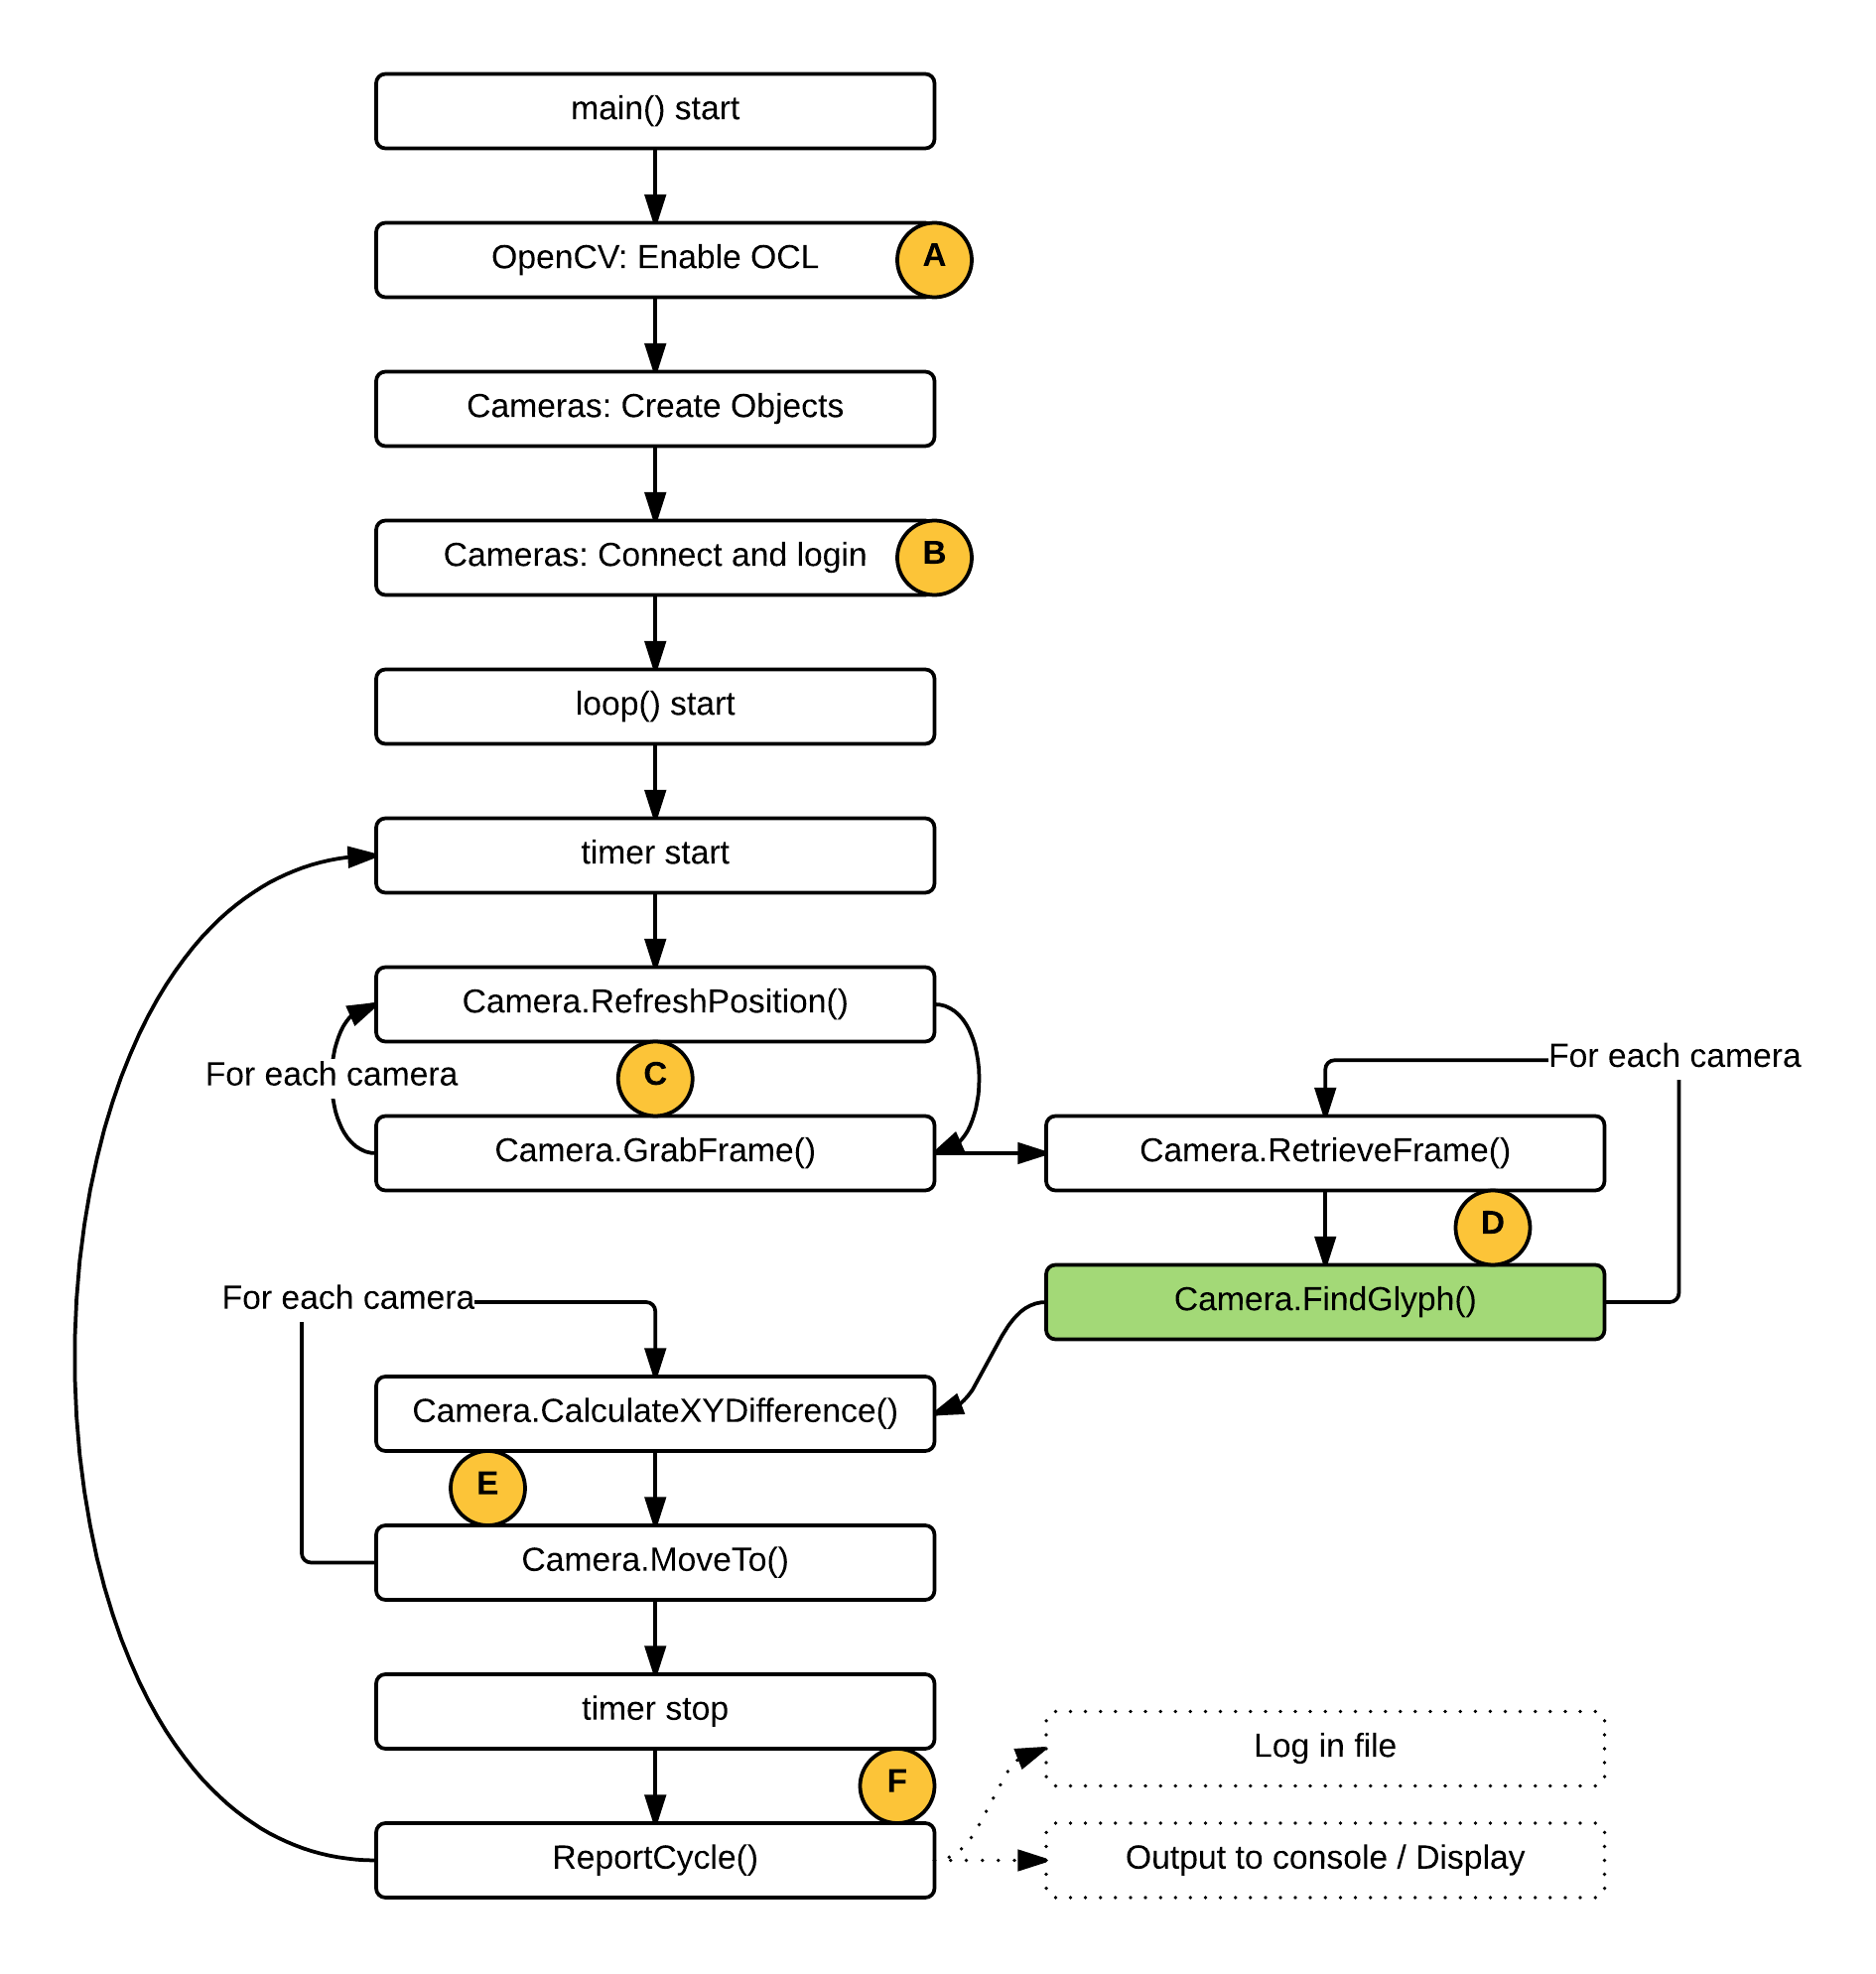
\includegraphics[width=1.0\textwidth]{software_design.png}
    \caption{Software flowchart as implemented. Source: Own work}
    \label{fig:software_design}
\end{figure}
\FloatBarrier

\subsubsection{Step A}
OpenCV 3.0 comes with a new transparent API, but we still have to enable the usage of OpenCL and verify that it is indeed working. This also gives us the opportunity to disable OpenCL to see how this affects the speed of our algorithm.
\subsubsection{Step B}
Each camera uses HTTP with Digest access authentication to prevent unauthorized access, which is an application of MD5 cryptographic hashing with nonce values to prevent replay attacks. The process of connecting to a camera and authenticating takes some time, so we do it once and increase the TCP parameters of the connection so that it is kept open. If we leave the TCP connection open, this should reduce the time needed for retrieving information in subsequent data transmissions. In order to create this connection, we query the camera for information while providing HTTP Digest information. The library we use is known as libcurl and more information about this open source project can be found at their webpage \citet{curl15}. Wireshark was used to find the authentication scheme.
\subsubsection{Step C}
Consider the loop in figure \ref{fig:software_design_c}.
Since we rely on receiving an image that is as up-to-date as possible, as well as the current camera parameters, we loop over each camera in our list. Camera.RefreshPosition() uses HTTP GET over the link previously established, in order to retrieve the following parameters, which were found using Wireshark:

\begin{itemize}
\item pan (float)
\item tilt (float)
\item zoom (integer)
\item iris (integer)
\item focus (integer)
\item autofocus (on/off)
\item autoiris (on/off)
\end{itemize}

Afterwards, we use OpenCV to grab the most recent frame from the MJPEG stream, and store this together with the most current timestamp. By using VideoCapture::grab(), we postpone decoding of the frame until a later stage. We do this to minimize the time-difference between two captured images from two different cameras.

\begin{figure}[ht]
    \centering
    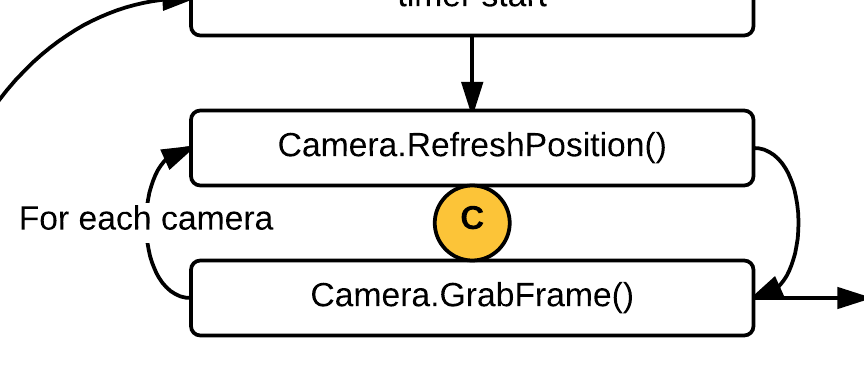
\includegraphics[width=0.8\textwidth]{software_design_c.png}
    \caption{Part C of flowchart. Source: Own work}
    \label{fig:software_design_c}
\end{figure}
\FloatBarrier


\subsubsection{Step D}
Consider the loop in figure \ref{fig:software_design_d}. We have in the last step gathered both images, positions and timestamp from the cameras. Now, we let OpenCV decode the images and then we run the glyph finding algorithm on each of these.
\begin{figure}[ht]
    \centering
    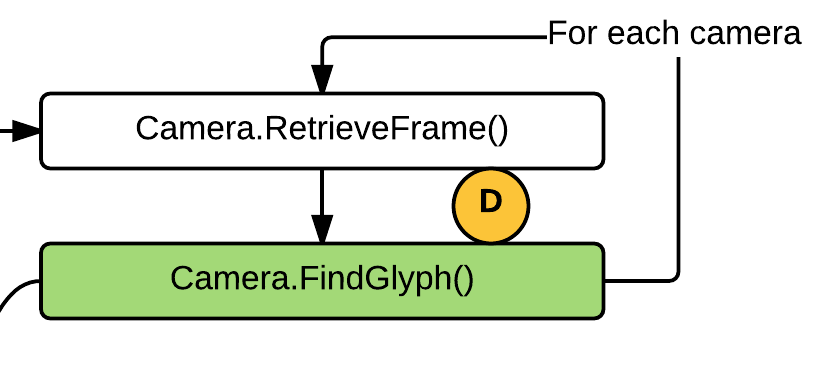
\includegraphics[width=0.8\textwidth]{software_design_d.png}
    \caption{Part D of flowchart. Source: Own work}
    \label{fig:software_design_d}
\end{figure}
\FloatBarrier

\subsubsection{Step E}
Consider the loop in figure \ref{fig:software_design_e}. Using the center of the glyph distance from the target pixel on the image, we calculate the difference and move the camera towards this position. This step can be made more advanced by implementing various controllers, but for this thesis, it remains a Proportional controller. The Camera.MoveTo() method uses HTTP to engage the PTZ camera.
\begin{figure}[ht]
    \centering
    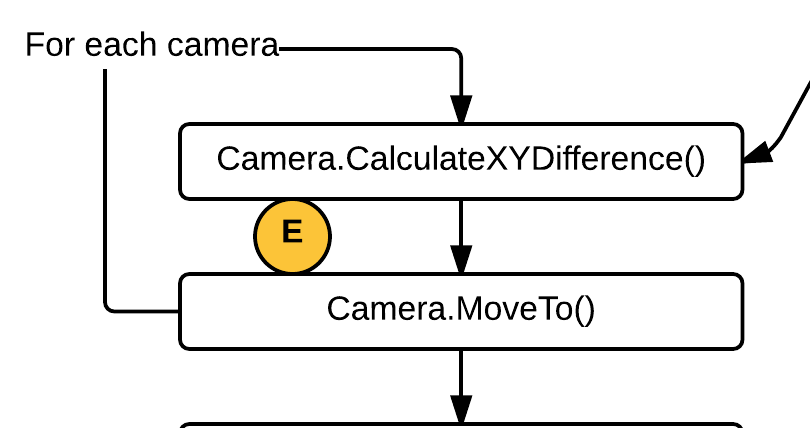
\includegraphics[width=0.8\textwidth]{software_design_e.png}
    \caption{Part E of flowchart. Source: Own work}
    \label{fig:software_design_e}
\end{figure}
\FloatBarrier

\subsubsection{Step F}
In \ref{fig:software_design_e}, we are now at the end of a cycle. The time spent on this cycle as well as other useful data is logged to a file. The same information can be presented on an augmented reality screen. A new cycle begins.
\begin{figure}[ht]
    \centering
    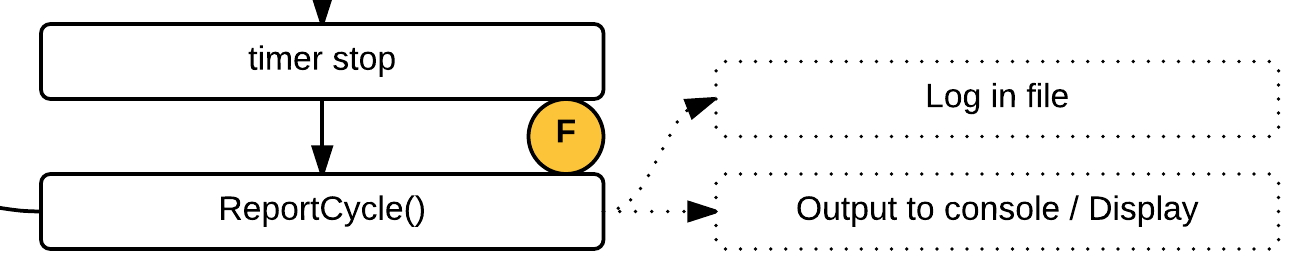
\includegraphics[width=1.0\textwidth]{software_design_f.png}
    \caption{Part F of flowchart. Source: Own work}
    \label{fig:software_design_f}
\end{figure}
\FloatBarrier

\subsection{Analysis of dataset for robustness in weather conditions}
Based on work done in the project thesis, a Python program using OpenCV 2 was created. Its purpose was to analyse pictures captured over the span of a year, from the MHWirth test tower located at Dvergsnes, Kristiansand.
\begin{equation}
58h 08min 18.3sec N 8h 04min 17.6sec E
\end{equation}

The dataset was gathered using another Python program written and deployed around christmas 2014, which at 15-minute intervals, captured images from a handful of CCTV cameras in the tower and stored them on a local server.

Located at various locations in the fifty meters tall test tower, the idea was that weather impacts would be strong.

As the CCTV cameras have built-in low-light mode, a period during the night is considered too dark for the algorithm to detect the glyph.

The program that gathered the pictures was running without supervision. A result of this was that some gaps of several days in the dataset exists.

Initially, all the pictures were stored as lossless 24-bit RGB Portable Network Graphics. However, after a few months, the amount of data being gathered was filling up the server storage. It was then decided to continue the data gathering using JPEG, which would cut the required storage space close to $\frac{1}{5}$ of the space required with PNG-24

\begin{equation}
\frac{pictures}{camera}=365 days\cdot 24\frac{h}{day}\cdot 4\frac{pics}{h}=35040
\end{equation}

\subsection{Tabletop setup for testing}
In order to rapidly develop and test the software in a controlled environment, a tabletop setup was created. The main PTZ camera was connected to the internet, while the USB webcamera was connected to the Linux server.

A custom built linear actuator was used to provide repeated linear motion. See Appendix \ref{ch:actuator} page \pageref{ch:actuator} for construction details.

A computer screen was used to roughly determine camera latency using a custom-built timer software. See figure \ref{fig:tabletop} for the full setup. The timer in use can be seen on figure \ref{fig:timer_in_use} where the camera looks at the screen which in turn displays the captured image. The difference between captured picture and displayed picture gives us a rough estimate of the latency we experience. In this case, we have close to 241 milliseconds of delay, nearly four frames per second.
\begin{equation}
9.274741s - 9.033639s = 0.241102s
\end{equation}

In order to protect the privacy of other students in the room, the back of the PTZ camera was covered.

\begin{figure}[ht]
    \centering
    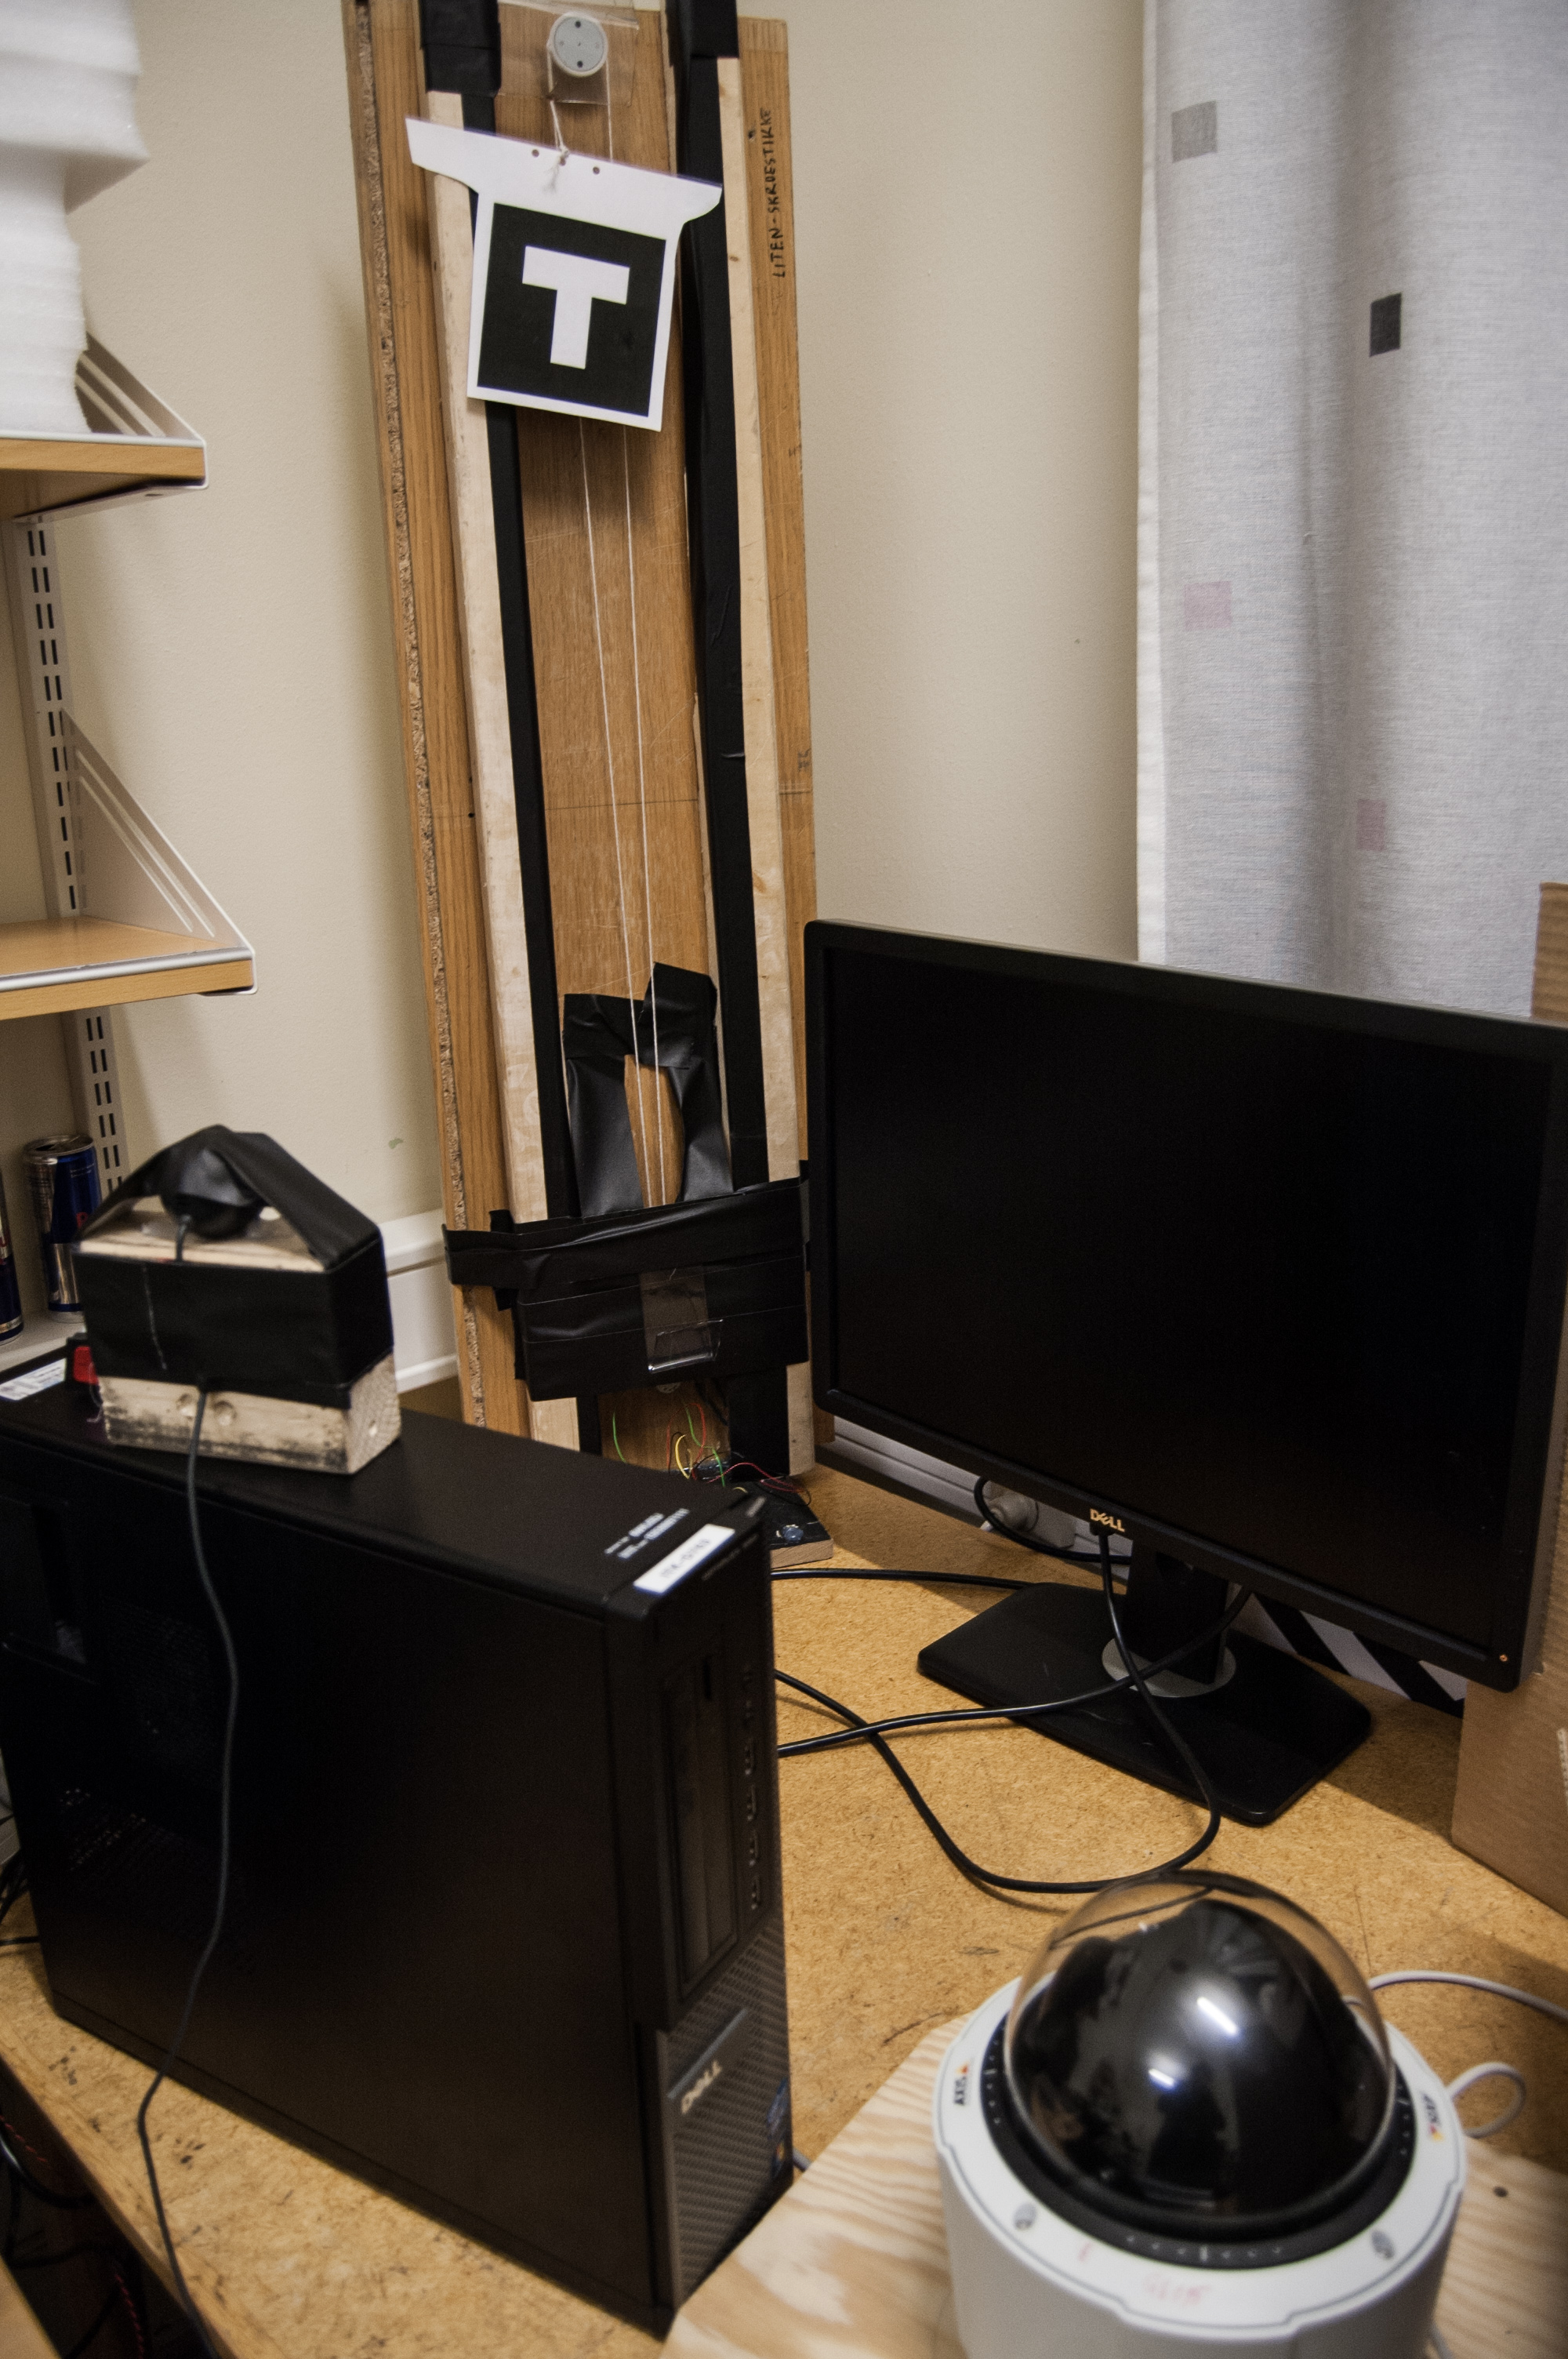
\includegraphics[width=0.8\textwidth]{tabletop.jpg}
    \caption{The tabletop setup. Source: Own work}
    \label{fig:tabletop}
\end{figure}

\begin{figure}[ht]
    \centering
    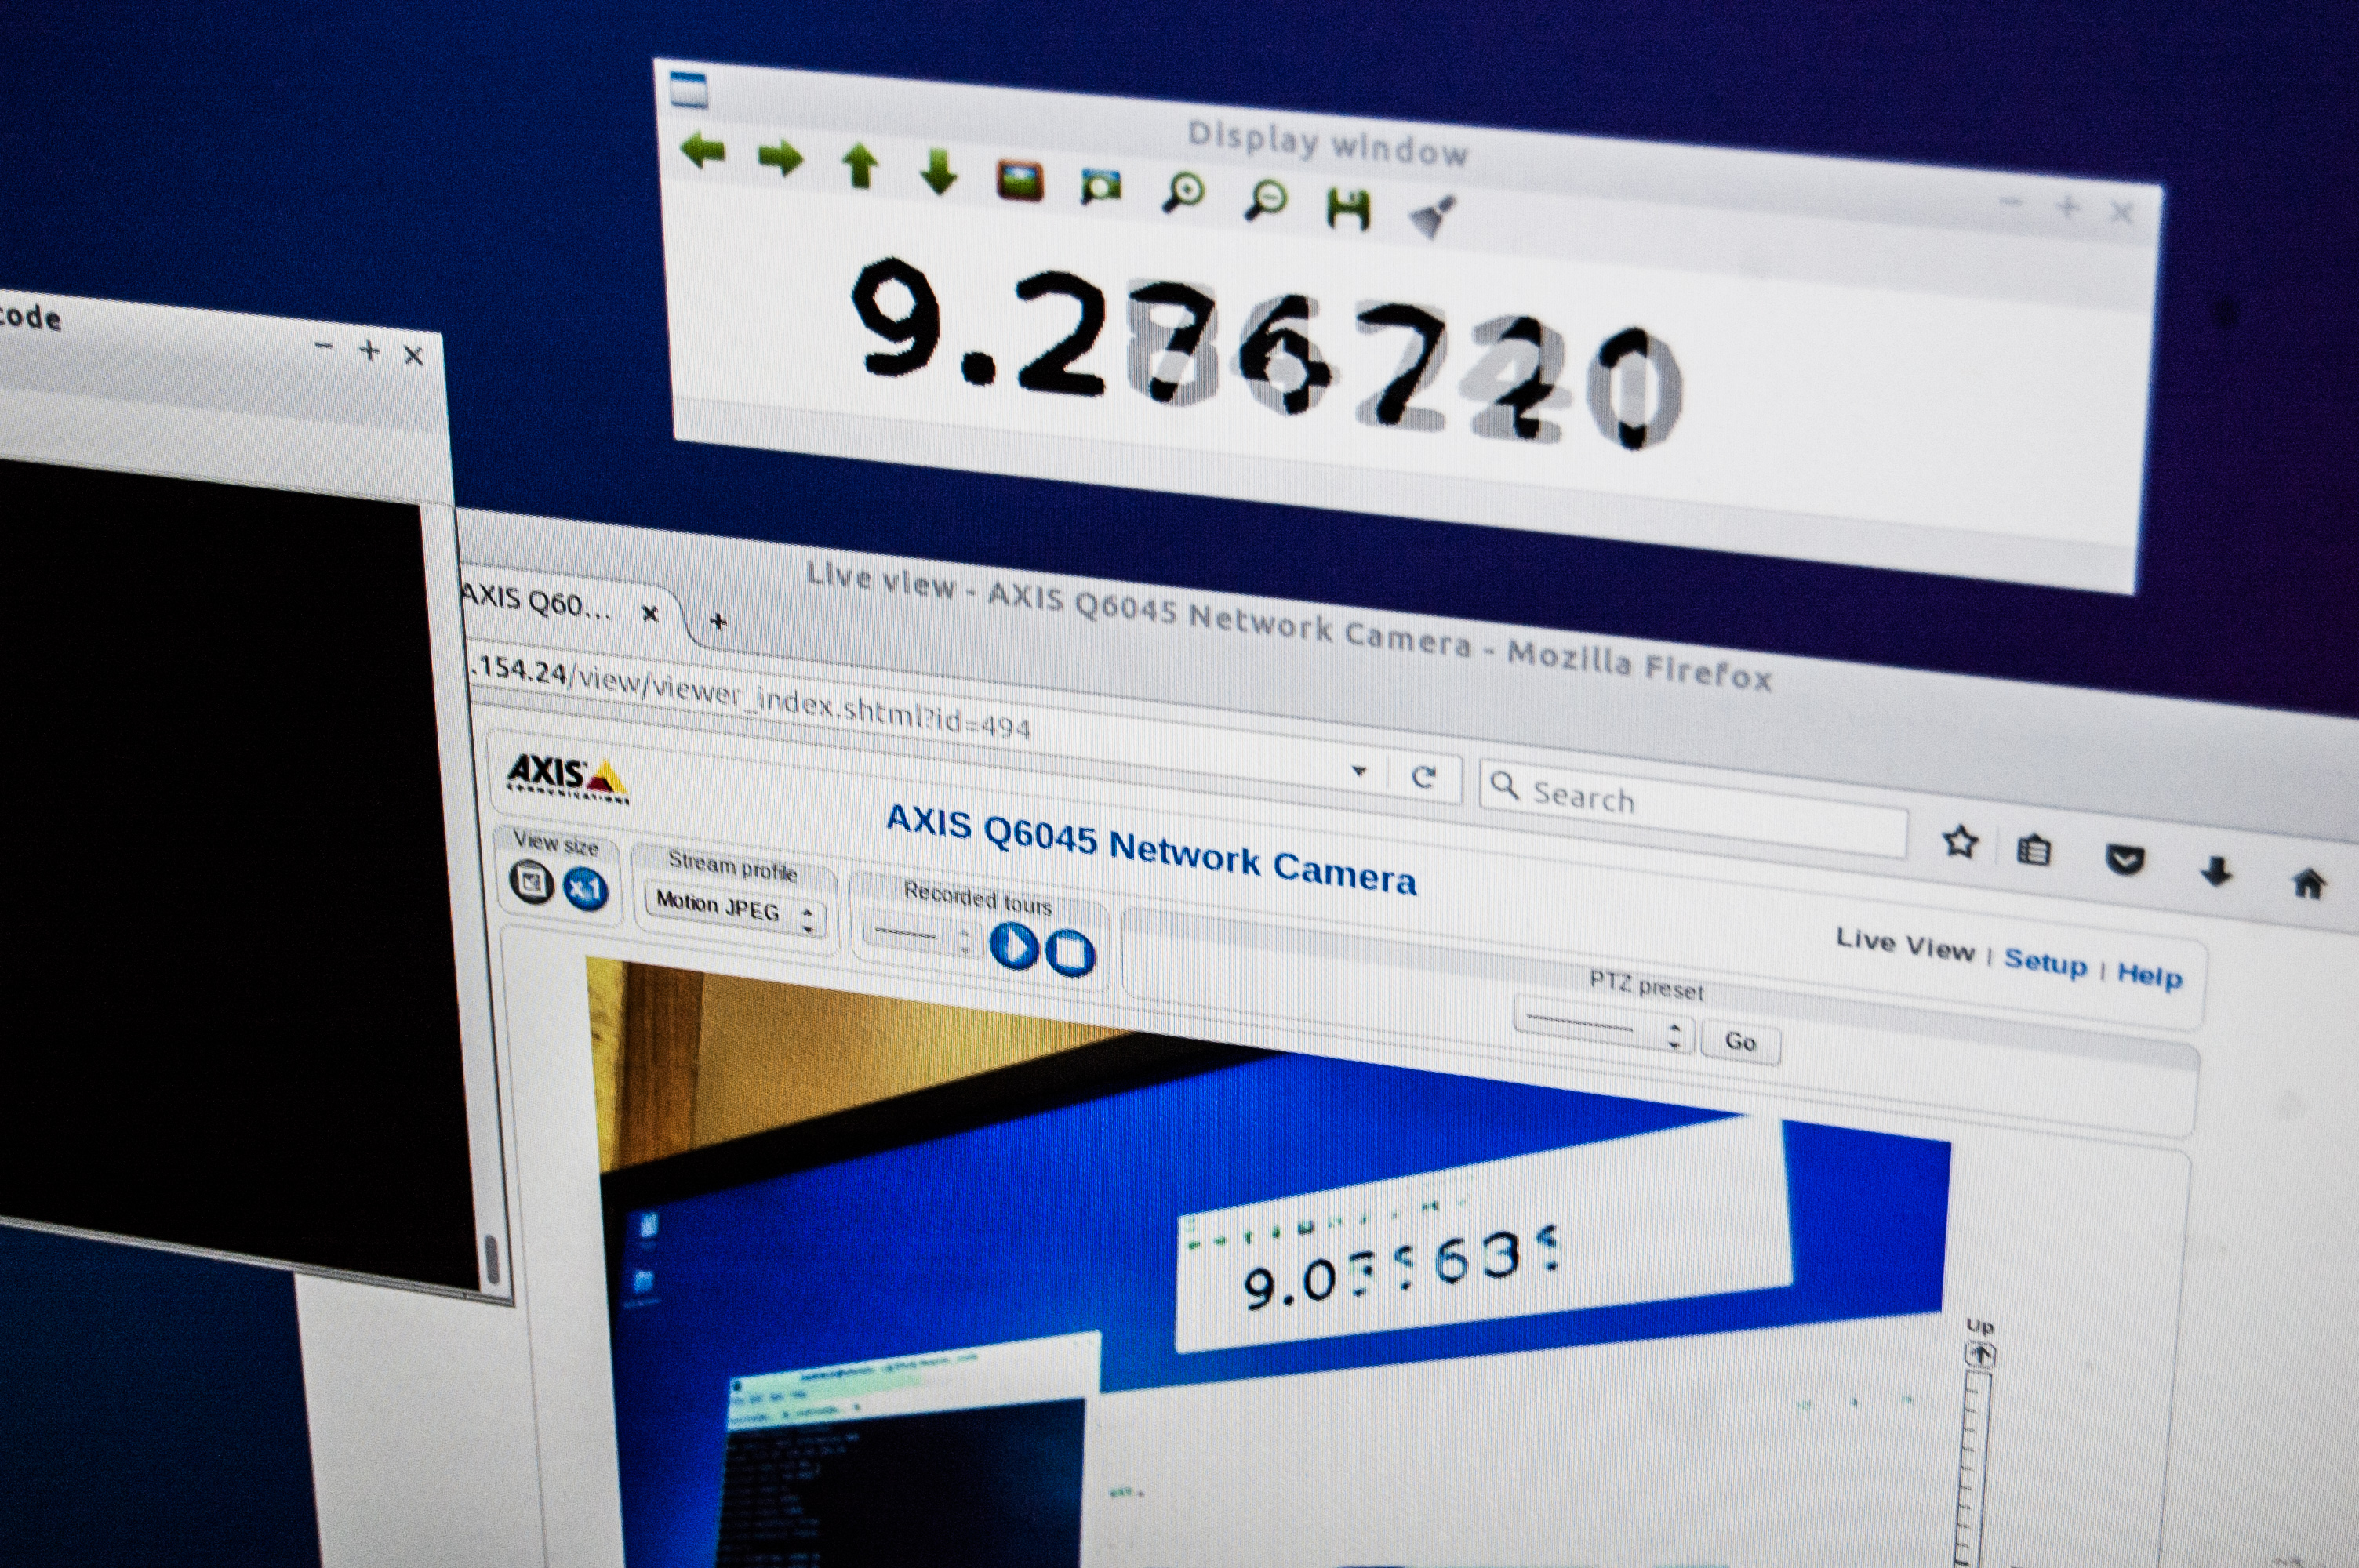
\includegraphics[width=0.8\textwidth]{timer_in_use.jpg}
    \caption{The timer software in use, showing 241 ms delay. Source: Own work}
    \label{fig:timer_in_use}
\end{figure}


\section{Tubular detection in fingerboard}
\subsection{Background}
Drilling pipes and risers, commonly called tubulars, are used to drill deep into the earth. These tubulars need to be stored in between their use in the drilling process. The most common method for short-term to mid-term storage is in groups of a few units in a machine called fingerboard, a part of the pipe handling equipment on a drilling rig.

\begin{figure}[ht]
    \centering
    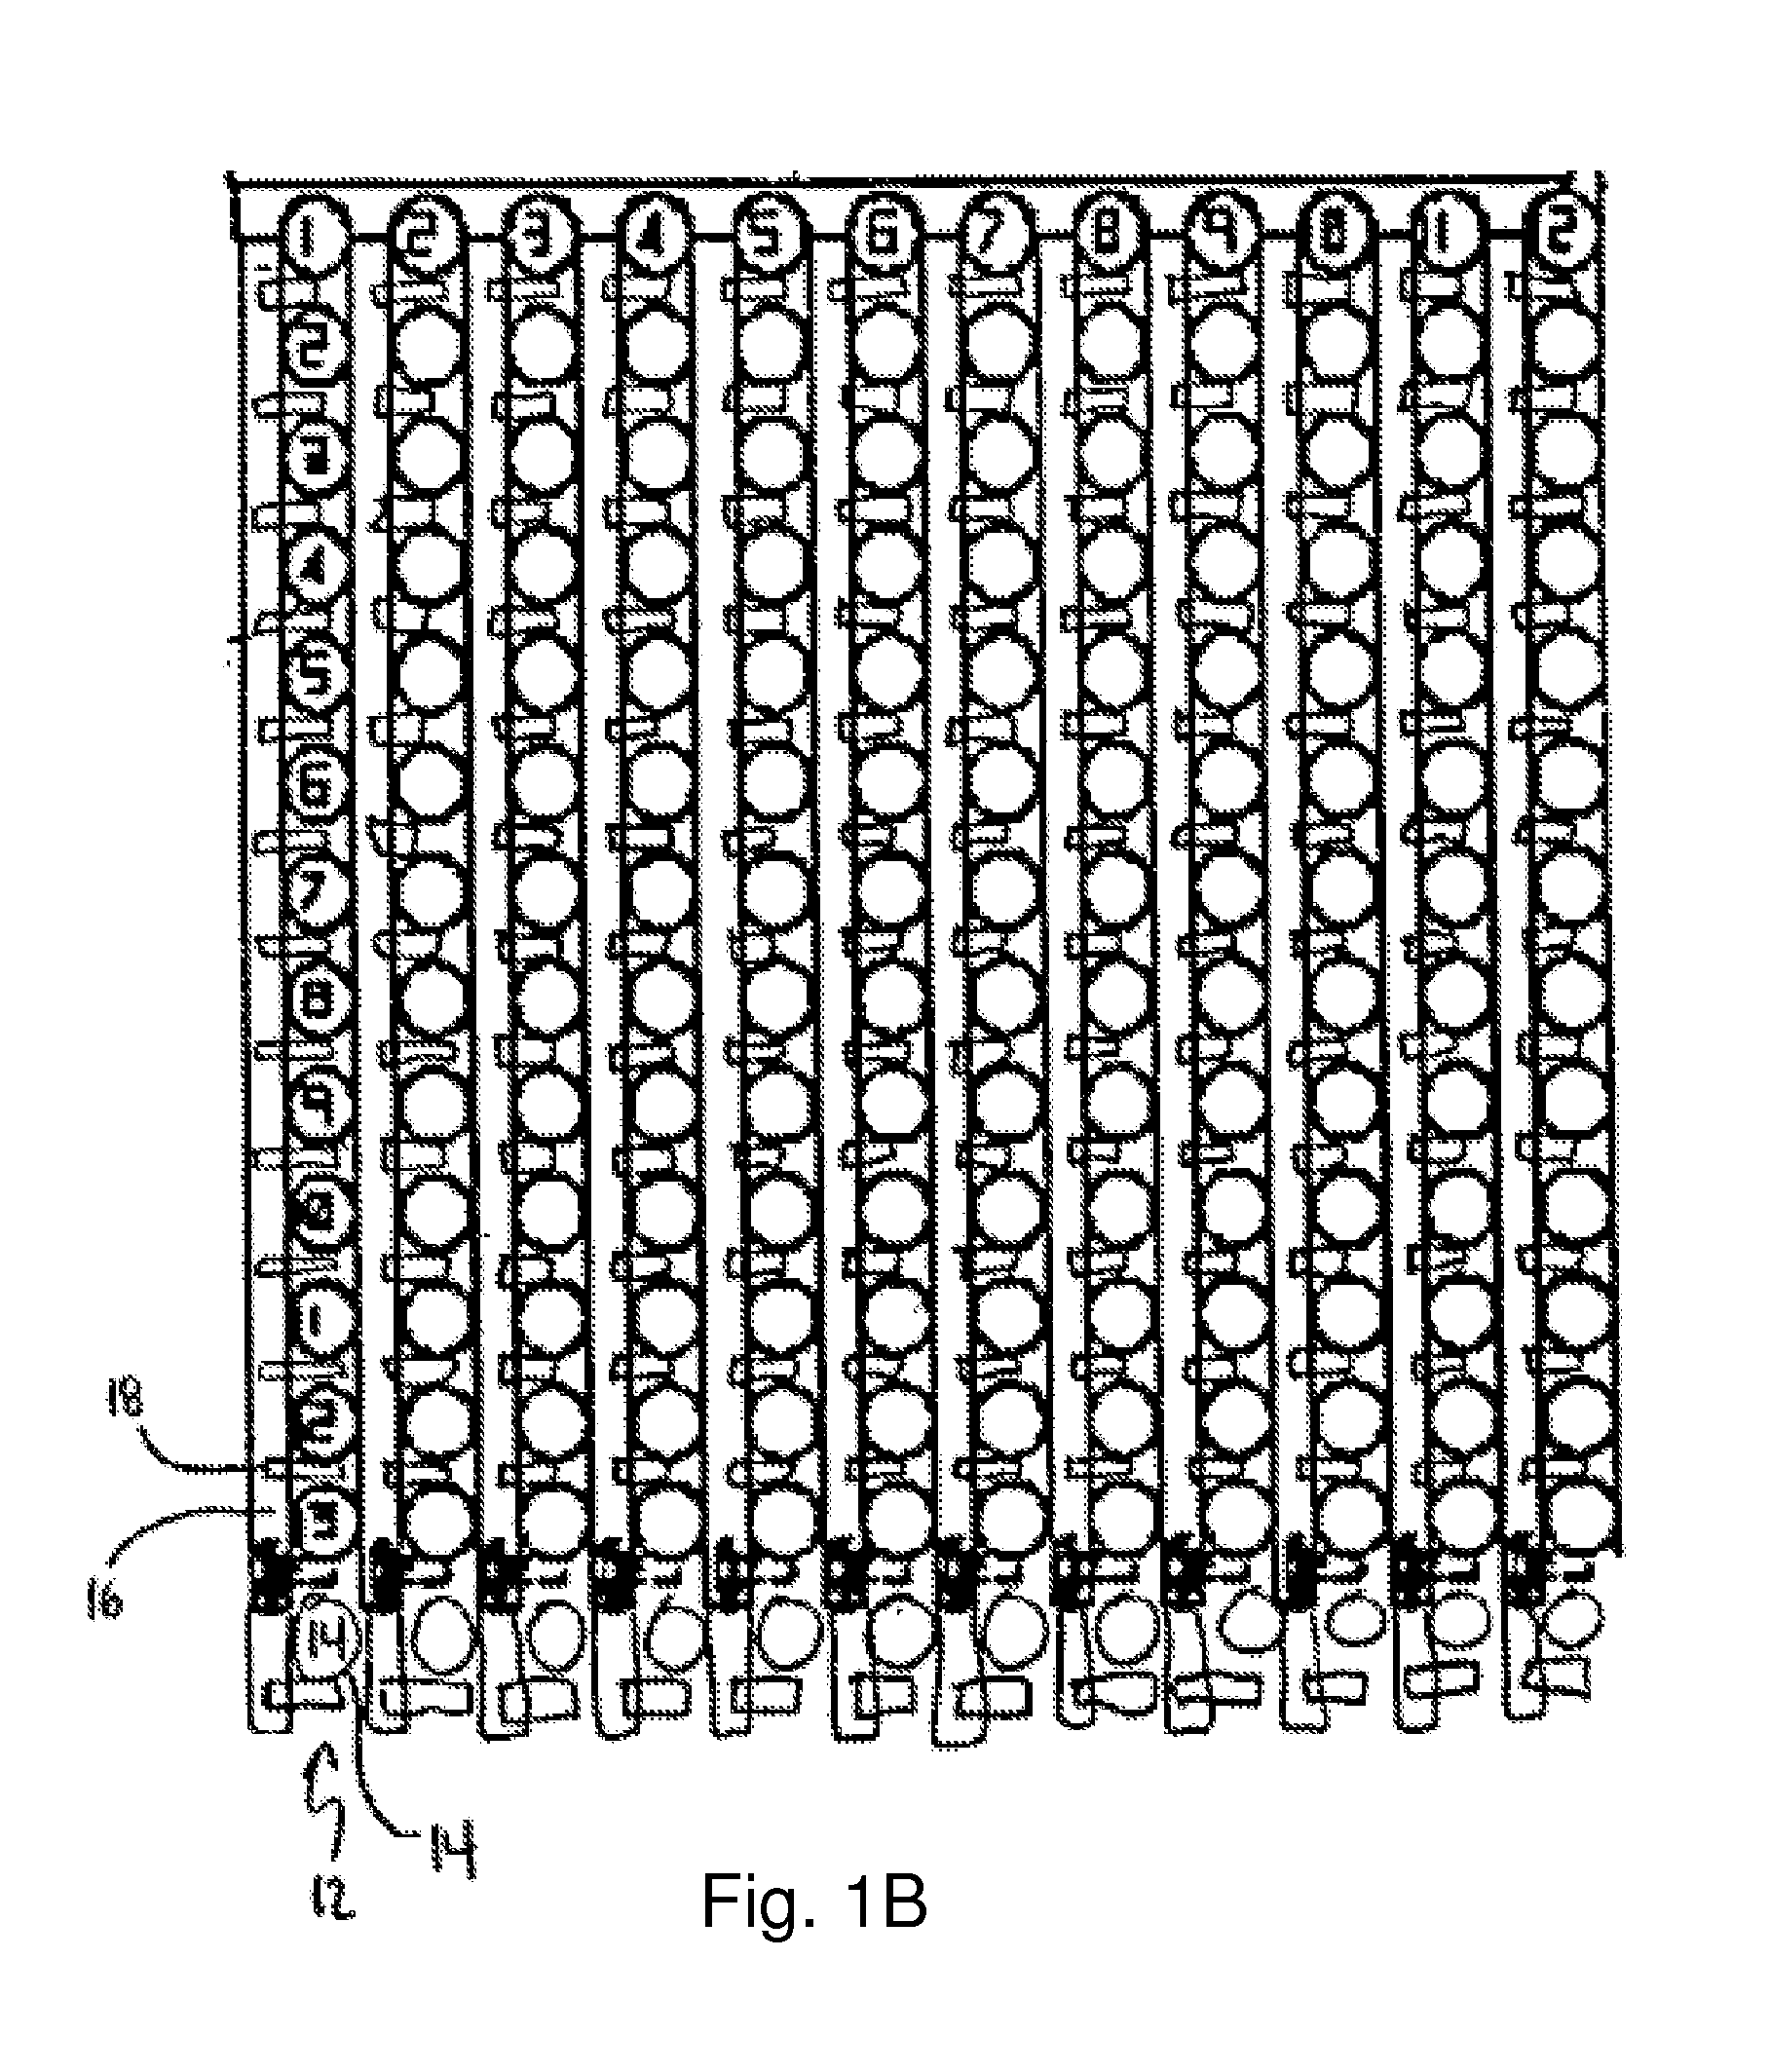
\includegraphics[width=0.8\textwidth]{fig_fb_cells_matrix.png}
    \caption{Diagram of a fingerboard with tubulars. Source:\cite{fig_fb_cells_matrix13}}
    \label{fig:fb_cells_matrix}
\end{figure}
\FloatBarrier

The first patent for a finger board was filed 1929 in the United States, and ever since, new patents that increase their capabilities have been filed. The latest ones use pneumatic cylinders to latch and secure tubulars in place, and a control system managing and tracking the pipes that should be in the fingerboard.

For more information regarding the history of the fingerboard, the reference list of a patent publicized February 2013 by \citet{pat_james13} is suggested. The patent in question discuss a method to report finger position data to the control system. With this feature, the control system becomes aware of its fingers, but knowing if a tubular exists in a given cell requires a fail-free logging of the actions done by other machines.

\begin{figure}[ht]
    \centering
    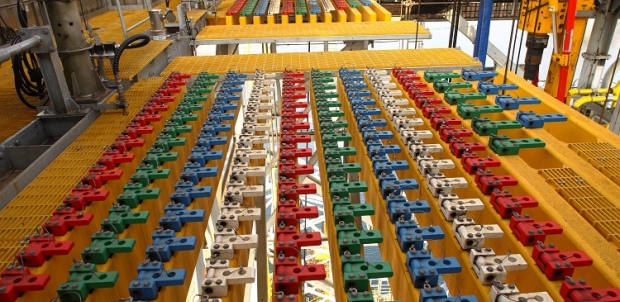
\includegraphics[width=0.8\textwidth]{fingerboard_tsc.jpg}
    \caption{Fingerboard without tubulars. Source:\cite{fig_fb_tsc15}}
    \label{fig:fb_tsc15}
\end{figure}
\FloatBarrier


\subsection{Goal of case study}
The goal of this case study is to draft an algorithm that can detect tubulars and associated parameters in a fingerboard. It is possible to develop the algorithm using more user-friendly click-and-drop vision packages, but the author settled on using OpenCV 3 because this does not require expensive and resource demanding software.

\subsection{Design of the machine vision algorithm}
The circularity of a circle can be described using the Heywood circularity factor. This factor can be used to narrow feature detection.

One possible solution involves using the Hough transform method to find ellipses in the picture, then analyze the region contained within to determine wheter the detected ellipse may outline a tubular. The algorithm implemented in OpenCV is based on a variant called the 2-1 Hough Transform by \citet{yuen90}. Partial occlusion of tubulars are a challenge.

Another more recent method of ellipse detection is presented by \citet{wang14} based on sorted merging. This algorithm is not yet implemented in OpenCV, but may be better at handling partial occlusion of the ellipses, and faster than the Hough transform based methods.

\begin{figure}[ht]
    \centering
    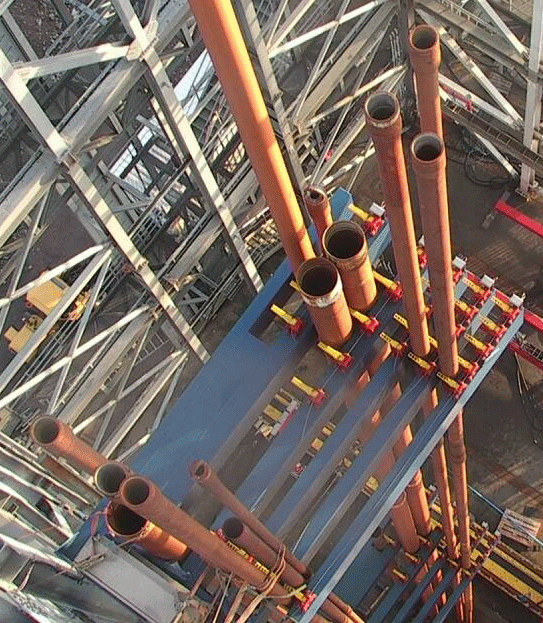
\includegraphics[width=0.8\textwidth]{fb_mhwirth.png}
    \caption{Fingerboard with tubulars. Source: Own work (MHWirth AS)}
    \label{fig:fb_mhwirth}
\end{figure}
\FloatBarrier

\begin{figure}[ht]
    \centering
    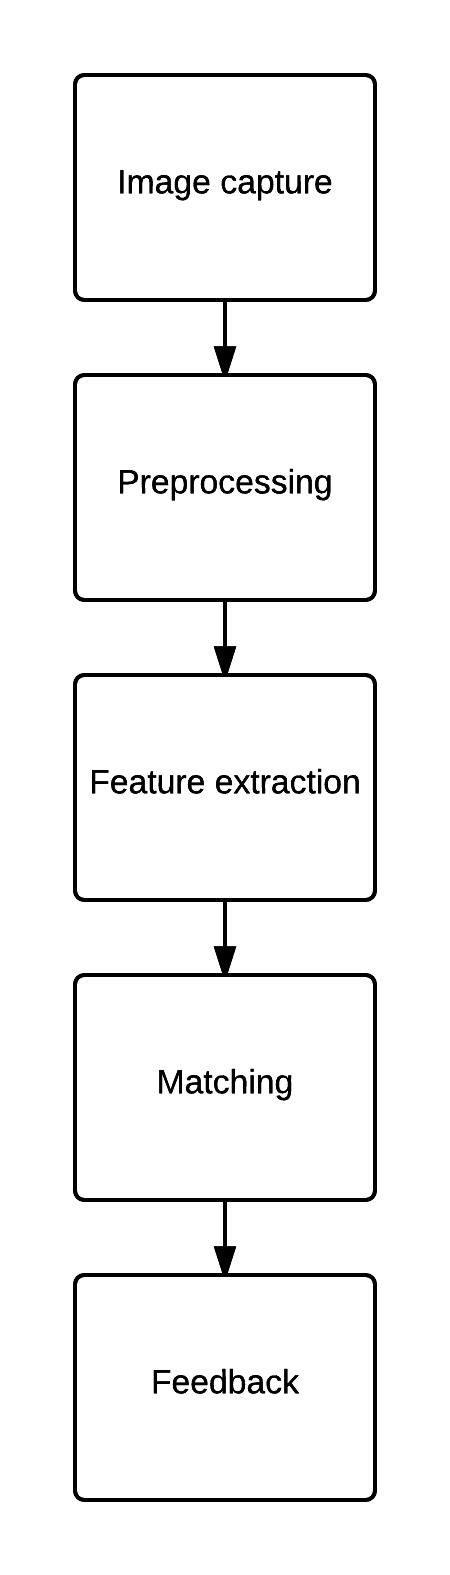
\includegraphics[width=0.3\textwidth]{alg_simple.png}
    \caption{A generic machine vision implementation before detailed description. Source: Own work}
    \label{fig:alg_simple}
\end{figure}
\FloatBarrier

We will now build up an algorithm as a hypothetical solution to the challenge, and the design choices made will be explained.

\subsubsection{Image capture}
The image is captured and stored with colors from the camera. In our case, we use the high-resolution AXIS Q6045 footage captured outdoors at MHWirth AS. For an actual implementation, any camera at a certain angle and position above the fingerboard will do. We are depending upon good lightning and decent weather, and we assume that no water droplets are found on the camera housing.

For the sake of comparison, a matrix that shows some mid-winter lightning conditions and how it affects the image, which in turn may break our algorithm. See figure \ref{fig:lightning_matrix}. The author's comments on this figure follows.

\paragraph{06:45} Only artificial light can be seen. The tubulars and the fingerboard are black, no features besides their orientation and if lucky, width of the pipe, can be extracted.

\paragraph{08:15} We can see the fingerboard and the tubulars, but the picture is filled with artifacts that appear in low-light conditions. It should be possible to extract features from this image, but it is sub-optimal.

\paragraph{10:00} The natural light from the sun is flat and thus, the image does not give us too much contrasts. The picture in itself should suffice to detect the tubulars.

\paragraph{13:15} The sun has now risen close to its max elevation above the horizon for the current date. A good amount of contrasts in the image makes this a good candidate for implementing a proof-of-concept algorithm.

\paragraph{17:00} Colors captured have shifted to a cold blue, the sun is almost gone. If we use colors to distinguish the tubular, this would provide a challenge, unless we adjust the white-balance.

\paragraph{17:15} The camera went into low-light mode, which removes the IR-filter. Any artificial light is also turned off at this time, leading to a dark muddy and noisy picture that is not good for our use.

\begin{figure}[ht]
    \centering
    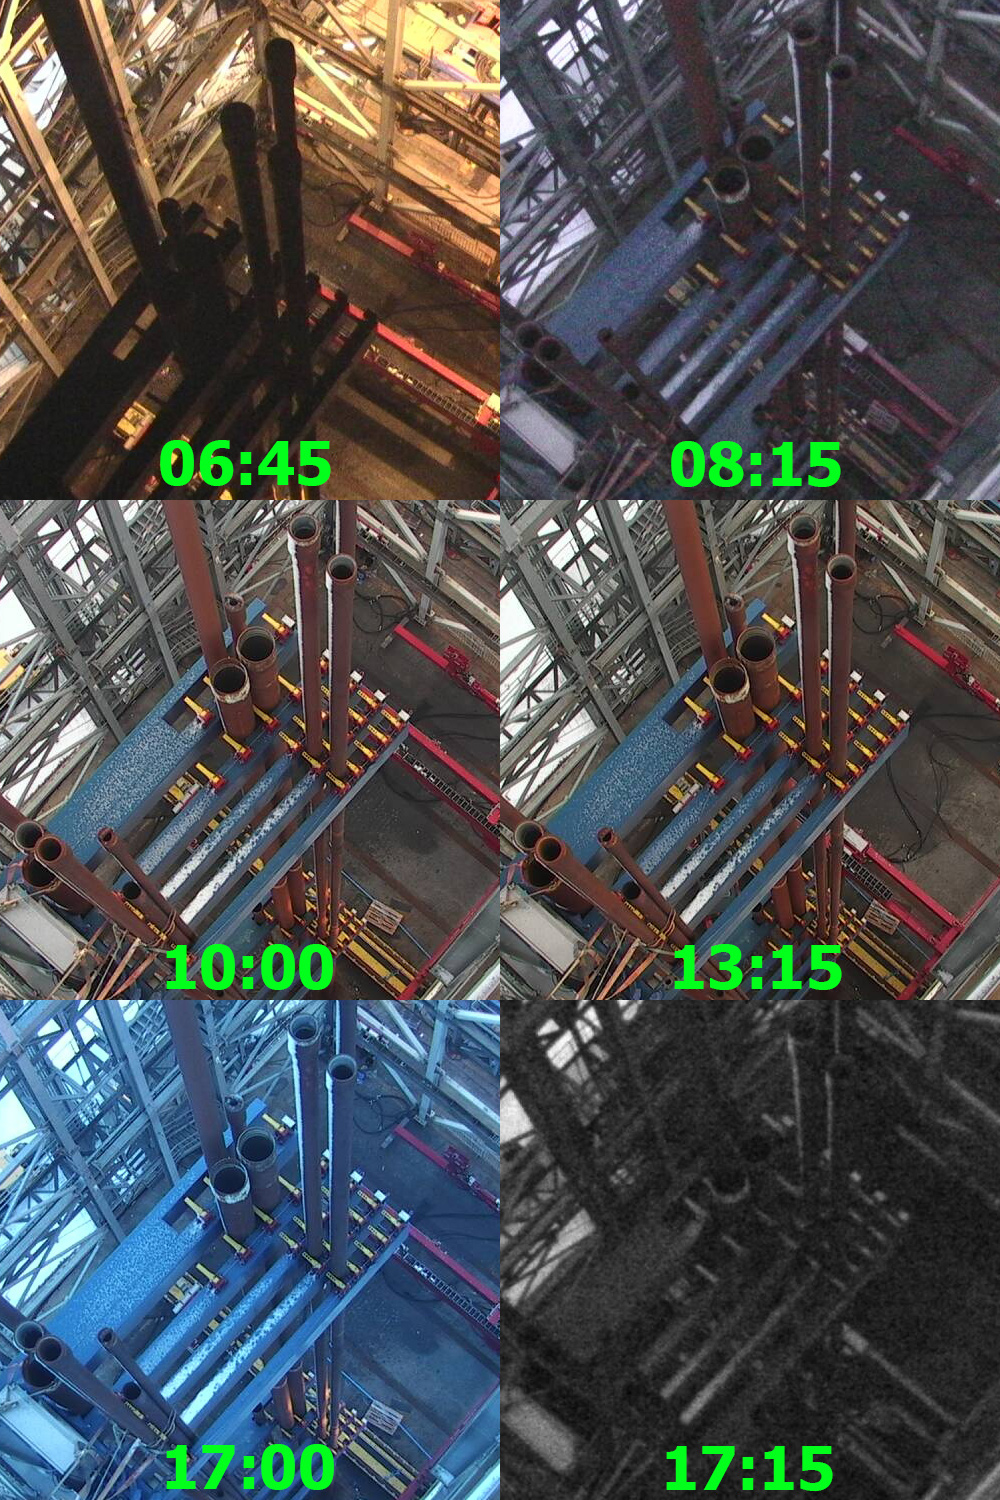
\includegraphics[width=0.85\textwidth]{lightning_matrix.jpg}
    \caption{Matrix of CCTV images to show differences in lightning. All times in UTC+1, captured 25th of January 2015. Source: Own work}
    \label{fig:lightning_matrix}
\end{figure}
\FloatBarrier

A thing to note is that the drilling floor on an offshore platform is not necessarily outdoors, but is partially sheltered from the environment, including natural light. This depends on the configuration. Machines may therefore move sheltered from natural light most of the time. Figure \ref{fig:wellcenter} shows a typical well center, partially in a partially sheltered area on an offshore oil platform. Figure \ref{fig:drillfloor_above} shows drillfloor as viewed from above, the fingerboards can be seen in the shade of the walls surrounding the tower.

\begin{figure}[ht]
    \centering
    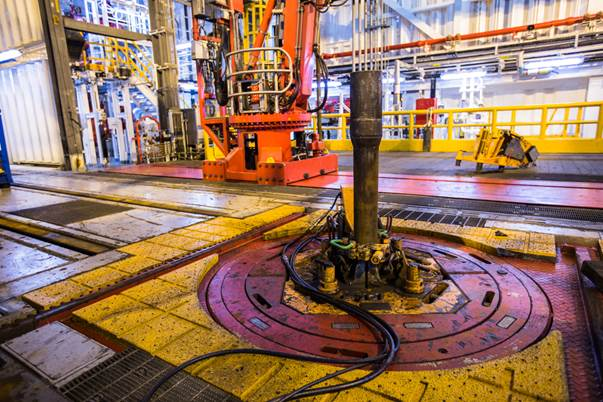
\includegraphics[width=1.0\textwidth]{drillfloor.jpg}
    \caption{Well center, at the base of the drill floor. Credit: Vegard Haugland, MHWirth AS, \citet{hauglandfoto15}}
    \label{fig:wellcenter}
\end{figure}
\FloatBarrier

\begin{figure}[ht]
    \centering
    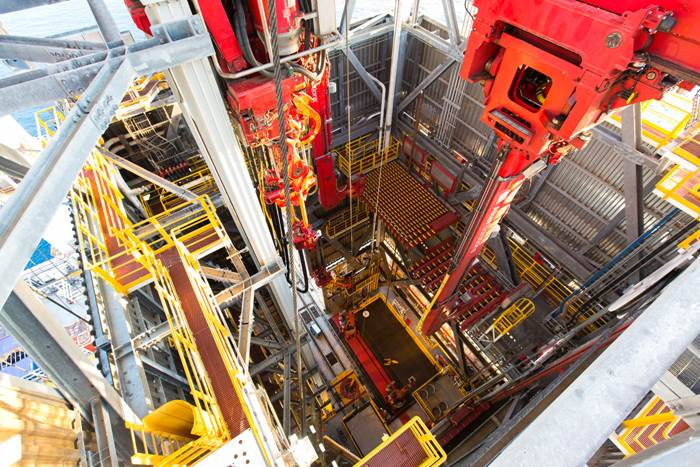
\includegraphics[width=1.0\textwidth]{drillfloor_above.jpg}
    \caption{Looking down on the drill floor from outside. Credit: Vegard Haugland, MHWirth AS, \citet{hauglandfoto15}}
    \label{fig:drillfloor_above}
\end{figure}
\FloatBarrier

Since the drilling floor seems to be sheltered, we will avoid using a picture with snow on it, as was seen in the matrix figure \ref{fig:lightning_matrix}, and instead we use figure \ref{fig:mhwirth_fingerboard_test_image}, taken 18th of January 15:00 UTC+1 in the MHWirth test tower.

\begin{figure}[ht]
    \centering
    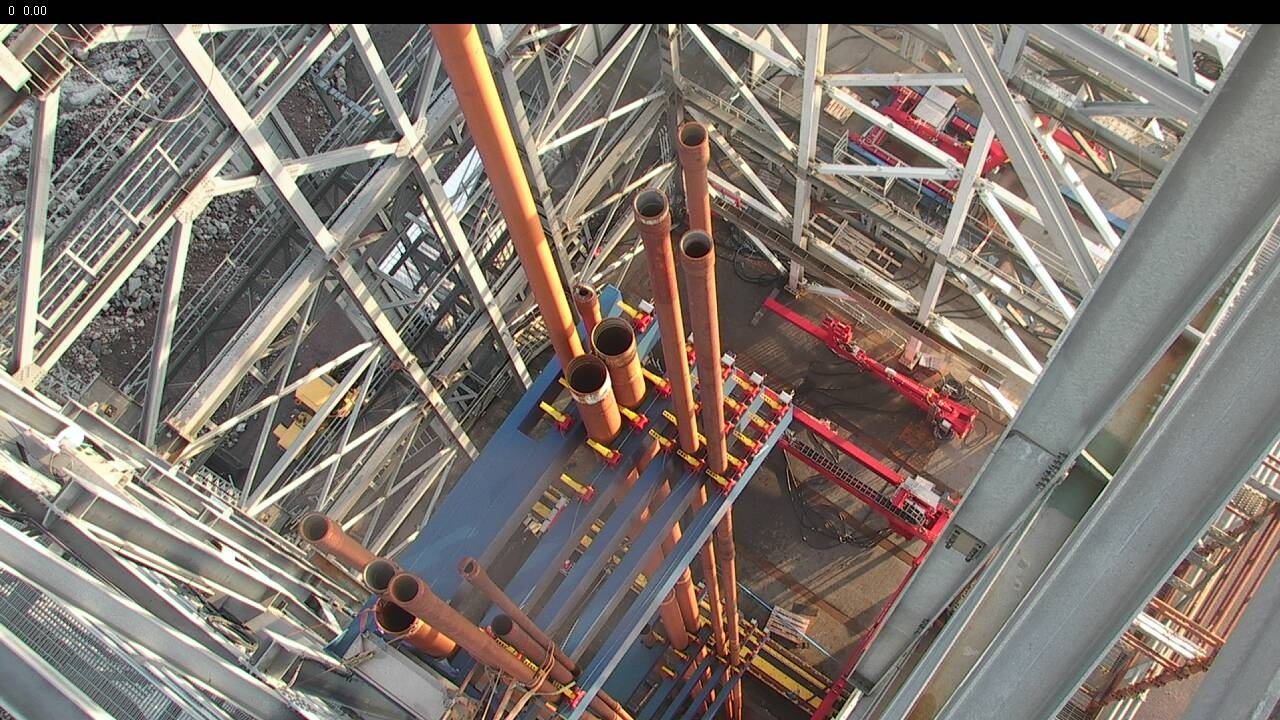
\includegraphics[width=1.0\textwidth]{mhwirth_fingerboard_test_image.jpg}
    \caption{Fingerboard tubular detection sample image, taken 18th of January 15:00 UTC+1. Source: Own work}
    \label{fig:mhwirth_fingerboard_test_image}
\end{figure}
\FloatBarrier


\subsubsection{Preprocessing}
After we have captured the image, we will need to preprocess it to maximize the performance of subsequent algorithms. The way we process the image depends on what we would like to do with it later on. One common step is to make a grayscale image, reducing colors that may not be needed. In this case, we will try to use what colors are found in the image, since the fingerboard, tubulars and fingers seem to have different colors. By using Adobe Photoshop or another image manipulation tool, we can quickly try out different blending methods, which may give us an idea of ways to improve the image to make it more suitable for known vision algorithms.

\begin{figure}[ht]
    \centering
    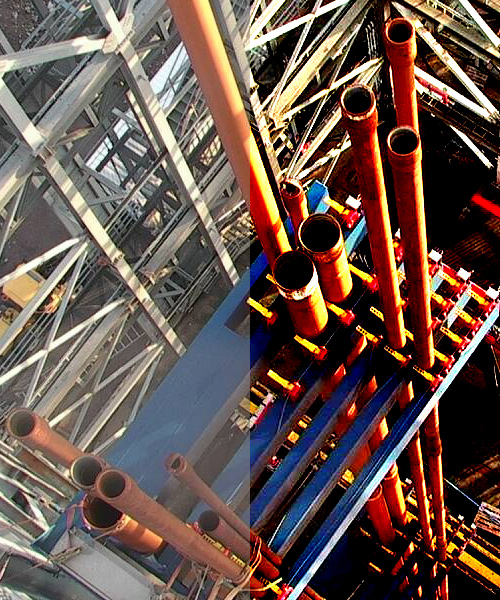
\includegraphics[width=1.0\textwidth]{linear_light.jpg}
    \caption{Linear light blending of color image using Adobe Photoshop. Source: Own work}
    \label{fig:linear_light}
\end{figure}
\FloatBarrier
\begin{figure}[ht]
    \centering
    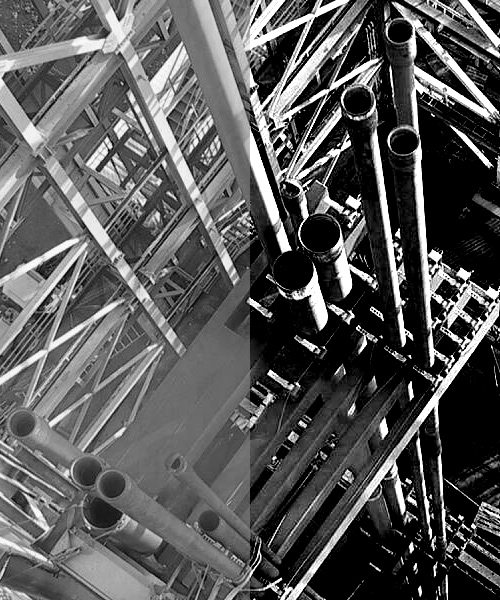
\includegraphics[width=1.0\textwidth]{linear_light_grayscale.jpg}
    \caption{Linear light blending of grayscale image using Adobe Photoshop. Source: Own work}
    \label{fig:linear_light_grayscale}
\end{figure}
\FloatBarrier

\subsubsection{Feature extraction}

\subsubsection{Matching}

\subsubsection{Feedback}